% ============================================================
%  XLA FACE PRIVACY SYSTEM — SLIDE THUYẾT TRÌNH
%  Nhóm: Đạt (Leader) · Khánh · Khoa
%  Môn: Xử Lý Ảnh Số · ĐH Phenikaa
%  XeLaTeX: fontspec + polyglossia (Vietnamese fix)
% ============================================================
\documentclass[aspectratio=169, 11pt]{beamer}

% ---- Theme: Boadilla (khác Madrid) ----
\usetheme{Boadilla}
\usefonttheme{professionalfonts}
\setbeamertemplate{navigation symbols}{}

% ---- Màu teal/coral (khác navy/red) ----
\definecolor{primary}{RGB}{0,105,92}
\definecolor{accent}{RGB}{224,87,45}
\definecolor{secbg}{RGB}{224,247,243}
\definecolor{codebg}{RGB}{248,248,248}
\definecolor{darkgreen}{RGB}{0,120,55}
\definecolor{gold}{RGB}{180,135,0}

\setbeamercolor{palette primary}{bg=primary, fg=white}
\setbeamercolor{palette secondary}{bg=primary!80, fg=white}
\setbeamercolor{palette tertiary}{bg=primary!60, fg=white}
\setbeamercolor{palette quaternary}{bg=primary!40, fg=white}
\setbeamercolor{frametitle}{bg=primary, fg=white}
\setbeamercolor{title}{fg=white}
\setbeamercolor{subtitle}{fg=white!85}
\setbeamercolor{block title}{bg=primary, fg=white}
\setbeamercolor{block body}{bg=secbg}
\setbeamercolor{block title alerted}{bg=accent, fg=white}
\setbeamercolor{block body alerted}{bg=accent!10}
\setbeamercolor{alerted text}{fg=accent}
\setbeamercolor{structure}{fg=primary}
\setbeamercolor{itemize item}{fg=primary}
\setbeamercolor{itemize subitem}{fg=accent}

% ---- XeLaTeX Font (FIX VIETNAMESE) ----
% KHÔNG dùng inputenc / fontenc / babel với XeLaTeX
\usepackage{fontspec}
\setsansfont{TeX Gyre Heros}
\setmonofont[Scale=0.85]{Latin Modern Mono}

% ---- Vietnamese (XeLaTeX cách đúng) ----
\usepackage{polyglossia}
\setmainlanguage{vietnamese}

% ---- Packages ----
\usepackage{listings}
\usepackage{booktabs}
\usepackage{tabularx}
\usepackage{array}
\usepackage{tikz}
\usetikzlibrary{shapes.geometric, arrows.meta, positioning, fit, backgrounds}
\usepackage{tcolorbox}
\tcbuselibrary{skins}
\usepackage{fontawesome5}
\usepackage{graphicx}
\usepackage{amsmath}
\usepackage{pifont}

\graphicspath{{./img/}{./image/}}

\newcommand{\cmark}{\textcolor{darkgreen}{\ding{51}}}
\newcommand{\xmark}{\textcolor{accent}{\ding{55}}}
\newcommand{\filecode}[1]{\texttt{\textcolor{primary!80!black}{\small #1}}}

% ---- Code style ----
\lstset{
  basicstyle=\ttfamily\footnotesize,
  keywordstyle=\color{primary}\bfseries,
  commentstyle=\color{darkgreen}\itshape,
  stringstyle=\color{accent},
  numbers=left, numberstyle=\tiny\color{gray}, numbersep=5pt,
  frame=tb, breaklines=true, showstringspaces=false,
  tabsize=2, backgroundcolor=\color{codebg},
}

% ---- TikZ styles ----
\tikzset{
  module/.style={rectangle, rounded corners=4pt,
    draw=primary, fill=secbg, thick,
    minimum height=0.85cm, minimum width=2.4cm,
    text width=2.2cm, align=center, font=\small},
  arrow/.style={->, >=Stealth, thick, color=primary},
  highlight/.style={rectangle, rounded corners=4pt,
    draw=accent, fill=accent!10, thick,
    minimum height=0.85cm, minimum width=2.4cm,
    text width=2.2cm, align=center, font=\small\bfseries},
  greenmod/.style={rectangle, rounded corners=4pt,
    draw=darkgreen, fill=darkgreen!10, thick,
    minimum height=0.85cm, minimum width=2.4cm,
    text width=2.2cm, align=center, font=\small},
}

% ---- Metadata ----
\title{XLA Face Privacy System}
\subtitle{Hệ Thống Camera Bảo Vệ Quyền Riêng Tư Khuôn Mặt}
\author{Đạt \textbullet\ Khánh \textbullet\ Khoa}
\institute{ĐH Phenikaa \textbullet\ KHDL\&AI}
\date{Xử Lý Ảnh Số · 2026}

% ============================================================
\begin{document}
% ============================================================

% ================================================================
%  FRAME 1 — TITLE
% ================================================================
\begin{frame}[plain]
\begin{tikzpicture}[remember picture, overlay]
  \fill[primary] (current page.north west)
    rectangle ([yshift=-0.44\paperheight] current page.north east);
  \node[text=white, anchor=north, font=\Large\bfseries]
    at ([yshift=-1.2cm] current page.north)
    {XLA Face Privacy System};
  \node[text=white!85, anchor=north, font=\normalsize]
    at ([yshift=-2.1cm] current page.north)
    {Hệ Thống Camera Bảo Vệ Quyền Riêng Tư Khuôn Mặt};
  \node[text=white!60, anchor=north, font=\small]
    at ([yshift=-2.9cm] current page.north)
    {Môn: Xử Lý Ảnh Số \quad\textbullet\quad ĐH Phenikaa};
\end{tikzpicture}

\vspace{3.7cm}
\begin{columns}[c]
\column{0.54\textwidth}
\begin{block}{\faUsers\ Nhóm thực hiện}
\footnotesize\renewcommand{\arraystretch}{1.4}
\begin{tabular}{lll}
\textbf{Vai trò} & \textbf{Họ tên} & \textbf{MSSV} \\
\hline
\textcolor{accent}{\textbf{Leader}} & \textcolor{accent}{\textbf{Hoàng Tiến Đạt}} & 23010864 \\
Backend & Nghiêm Xuân Khánh & 23010598 \\
Detection & Nguyễn Hữu Đăng Khoa & 23010901 \\
\end{tabular}
\end{block}
\column{0.42\textwidth}
\begin{block}{\faCog\ Công nghệ chính}
\footnotesize
\begin{itemize}
  \item Python 3.13 + FastAPI
  \item YOLOv11n-face + InsightFace
  \item AES-256-GCM + PBKDF2
  \item Lớp: KHDL\&AI
\end{itemize}
\end{block}
\end{columns}
\end{frame}

% ================================================================
%  FRAME 2 — AGENDA
% ================================================================
\begin{frame}{Nội Dung Thuyết Trình}
\begin{columns}[T]
\column{0.48\textwidth}
\begin{block}{\faList\ Phần 1 --- Tổng quan}
\begin{enumerate}\footnotesize
  \item Vấn đề \& Giải pháp
  \item Kiến trúc hệ thống
  \item Phân công nhiệm vụ
\end{enumerate}
\end{block}
\begin{block}{\faCog\ Phần 2 --- Kỹ thuật}
\begin{enumerate}\footnotesize\setcounter{enumi}{3}
  \item Phát hiện khuôn mặt (YOLOv11)
  \item Nhận diện thành viên (InsightFace)
  \item 6 chế độ ẩn danh hoá
  \item Backend \& Live Pipeline
\end{enumerate}
\end{block}
\column{0.48\textwidth}
\begin{block}{\faLock\ Phần 3 --- Bảo mật}
\begin{enumerate}\footnotesize\setcounter{enumi}{7}
  \item Mã hoá AES-256-GCM
  \item Admin authentication (PBKDF2)
\end{enumerate}
\end{block}
\begin{block}{\faDesktop\ Phần 4 --- Demo \& Kết quả}
\begin{enumerate}\footnotesize\setcounter{enumi}{9}
  \item Giao diện Admin \& User
  \item Kết quả benchmark
  \item Kết luận \& Câu hỏi
\end{enumerate}
\end{block}
\end{columns}
\end{frame}

% ================================================================
\section{Tổng Quan}
% ================================================================

% ---- FRAME 3: Vấn đề & Giải pháp ----
\begin{frame}{Vấn Đề \& Giải Pháp}
\begin{columns}[T]
\column{0.48\textwidth}
\begin{alertblock}{\faExclamationTriangle\ Thực trạng}
\begin{itemize}\footnotesize
  \item Camera an ninh ghi lại \textbf{tất cả mọi người}
  \item Khách bị nhận dạng \textbf{không có đồng ý}
  \item Vi phạm GDPR, BIPA, quyền riêng tư
  \item Dữ liệu khuôn mặt không mã hoá
\end{itemize}
\end{alertblock}

\begin{alertblock}{\faTimes\ Hai thái cực đều sai}
\footnotesize\begin{center}
\begin{tabular}{cc}
\textbf{Ghi thô} & \textbf{Xoá hết} \\
\hline
\xmark\ Lộ danh tính & \xmark\ Mất bằng chứng \\
\end{tabular}
\end{center}
\end{alertblock}

\column{0.48\textwidth}
\begin{block}{\faLightbulb\ Giải pháp: Privacy by Default}
\begin{itemize}\footnotesize
  \item \textbf{Luồng công khai:} Video blur người lạ, xem tự do
  \item \textbf{Luồng bảo mật:} Video gốc mã hoá AES-256-GCM
  \item Thành viên đã đăng ký: \textcolor{darkgreen}{\textbf{không bị che}}
  \item Người chưa đăng ký: \textcolor{accent}{\textbf{ẩn danh hoàn toàn}}
\end{itemize}
\end{block}

\begin{block}{\faCheckCircle\ Mục tiêu}
\centering\footnotesize
\textbf{Bảo vệ quyền riêng tư}\\
mà \textbf{vẫn giữ nguyên bằng chứng}
\end{block}
\end{columns}
\end{frame}

% ---- FRAME 4: Kiến trúc tổng thể ----
\begin{frame}{Kiến Trúc Hệ Thống}
\begin{center}
\begin{tikzpicture}[node distance=0.55cm and 0.7cm,
    scale=0.80, every node/.style={scale=0.80}]

  \node[module, minimum width=1.9cm] (cam) {\faCamera\\Camera};
  \node[module, right=0.65cm of cam, minimum width=2.2cm] (yolo)
    {\textbf{YOLOv11n}\\Face Detect};
  \node[module, right=0.65cm of yolo, minimum width=2.2cm] (if)
    {\textbf{InsightFace}\\buffalo\_l\\512-dim};
  \node[module, right=0.65cm of if, minimum width=2.2cm] (db)
    {\textbf{FamilyDB}\\cosine match};

  \node[greenmod, below=1.3cm of yolo, xshift=1.1cm, minimum width=2.4cm] (blur)
    {\faEyeSlash\ \textbf{Blur}\\7 modes\\.mp4 public};
  \node[highlight, below=1.3cm of if, xshift=1.7cm, minimum width=2.4cm] (enc)
    {\faLock\ \textbf{AES-256}\\Video gốc\\.enc private};

  \node[draw=gray, fill=gray!8, rounded corners, below=0.65cm of blur,
        minimum width=5.5cm, minimum height=0.7cm,
        font=\small, text width=5.2cm, align=center] (fe)
    {\faGlobe\ \textbf{Web Frontend} (FastAPI :8000)};

  \draw[arrow] (cam)  -- (yolo);
  \draw[arrow] (yolo) -- (if);
  \draw[arrow] (if)   -- (db);
  \draw[arrow] (db)   -- ++(0,-0.6) -| (blur);
  \draw[arrow] (db)   -- ++(0,-0.6) -| (enc);
  \draw[arrow] (blur.south) -- (fe.north);
  \draw[->, dashed, accent, >=Stealth, thick] (enc.south) -- ++(0,-0.5) -| (fe.east);

  \node[font=\tiny\color{darkgreen}, above=0.05cm of blur.north] {Người lạ};
  \node[font=\tiny\color{accent},    above=0.05cm of enc.north]  {Admin only};
\end{tikzpicture}
\end{center}
\end{frame}

% ---- FRAME 5: Phân công ----
\begin{frame}{Phân Công Nhiệm Vụ}
\begin{columns}[T]
\column{0.32\textwidth}
\begin{block}{\textcolor{accent}{\faUserTie\ Đạt — Leader}}
\footnotesize\textbf{Security \& Blur Engine}
\begin{itemize}
  \item \filecode{privacy.py} --- 7 mode
  \item \filecode{clip\_recorder.py} --- AES
  \item \filecode{admin\_auth.py} --- PBKDF2
  \item \filecode{face\_lock.py}
  \item \filecode{anonymizer\_backend.py}
\end{itemize}
\end{block}
\column{0.32\textwidth}
\begin{block}{\faUser\ Khánh — Backend}
\footnotesize\textbf{API \& Pipeline}
\begin{itemize}
  \item \filecode{app\_api.py} 1700+ dòng
  \item \filecode{backend\_api.py}
  \item \filecode{run\_phone\_cam.py}
  \item \filecode{bbox\_smoother.py}
  \item \filecode{frontend/*.html} 6 trang
\end{itemize}
\end{block}
\column{0.32\textwidth}
\begin{block}{\faUser\ Khoa — Detection}
\footnotesize\textbf{AI \& Database}
\begin{itemize}
  \item \filecode{detector.py} YOLOv11
  \item \filecode{face\_recognition.py}
  \item \filecode{family\_database.py}
  \item \filecode{yolov11n-face.pt}
  \item 100 mẫu ảnh/người
\end{itemize}
\end{block}
\end{columns}

\vspace{0.3em}
\begin{center}\footnotesize
\begin{tabular}{llll}
\toprule
\textbf{Thành phần} & \textbf{Công nghệ} & \textbf{Phiên bản} & \textbf{Vai trò} \\
\midrule
Detection & Ultralytics YOLO & v11n-face & Bounding box khuôn mặt \\
Recognition & InsightFace & buffalo\_l & Embedding 512 chiều \\
Backend & FastAPI + Uvicorn & $\geq$0.115 & REST + WebSocket \\
Crypto & cryptography & $\geq$43.0 & AES-GCM + PBKDF2 \\
\bottomrule
\end{tabular}
\end{center}
\end{frame}

% ================================================================
\section{AI: Detection \& Recognition}
% ================================================================

% ---- FRAME 6: YOLOv11 ----
\begin{frame}[fragile]{YOLOv11n-face --- Phát Hiện Khuôn Mặt}
\begin{columns}[T]
\column{0.5\textwidth}
\begin{block}{\faThumbsUp\ Lý do chọn YOLOv11n}
\begin{itemize}\footnotesize
  \item \textbf{Nano} --- tối ưu CPU, không cần GPU
  \item Fine-tuned đặc biệt cho face detection
  \item Non-Max Suppression tích hợp sẵn
  \item \texttt{detect\_every=2}: bỏ qua 1 frame/2\\
        $\Rightarrow$ giảm 50\% compute cost
\end{itemize}
\end{block}
\begin{block}{\faCogs\ Thông số cấu hình}
\footnotesize
\begin{tabular}{ll}
\texttt{imgsz}  & 512 px (inference size) \\
\texttt{conf}   & 0.35 (min confidence) \\
\texttt{iou}    & 0.50 (NMS threshold) \\
\texttt{detect\_every} & 2 (skip alternate frames) \\
\end{tabular}
\end{block}
\column{0.46\textwidth}
\begin{lstlisting}[language=Python, caption={detector.py}]
class FaceDetector:
  def detect_faces(self, frame):
    results = self.model(
      frame,
      imgsz=512,
      conf=0.35,
      iou=0.50,
      verbose=False,
    )
    boxes = []
    for r in results:
      for box in r.boxes:
        x1,y1,x2,y2 = map(
          int, box.xyxy[0])
        boxes.append(
          [x1,y1,x2-x1,y2-y1])
    return boxes
\end{lstlisting}
\end{columns}
\end{frame}

% ---- FRAME 7: InsightFace ----
\begin{frame}{InsightFace Buffalo-L --- Nhận Diện Thành Viên}
\begin{columns}[T]
\column{0.5\textwidth}
\begin{block}{\faBrain\ Embedding 512 chiều}
\begin{itemize}\footnotesize
  \item Model \textbf{buffalo\_l}: state-of-the-art recognition
  \item Vector 512 chiều = ``vân tay số'' khuôn mặt
  \item Cosine similarity từ $-1$ đến $+1$
  \item Threshold \textbf{0.35}:
  \begin{itemize}\scriptsize
    \item $> 0.35$ $\Rightarrow$ thành viên $\Rightarrow$ \textcolor{darkgreen}{\textbf{không blur}}
    \item $\leq 0.35$ $\Rightarrow$ người lạ $\Rightarrow$ \textcolor{accent}{\textbf{blur}}
  \end{itemize}
\end{itemize}
\end{block}
\begin{block}{\faChartBar\ Vectorized Matching}
\footnotesize
$$\text{sim}(a,b) = \frac{a \cdot b}{\|a\| \cdot \|b\|}$$
So sánh 1 lần với toàn bộ embedding matrix\\
$\Rightarrow$ O(n), không cần vòng lặp Python
\end{block}
\column{0.46\textwidth}
\begin{block}{\faDatabase\ Database hiện tại}
\footnotesize\renewcommand{\arraystretch}{1.4}
\begin{tabular}{lcc}
\textbf{Thành viên} & \textbf{Mẫu} & \textbf{Threshold} \\
\hline
Hoàng Tiến Đạt & 100 & 0.35 \\
Nguyễn Hữu Đăng Khoa & 100 & 0.35 \\
\end{tabular}
\end{block}
\begin{alertblock}{\faLightbulb\ Tại sao 100 mẫu?}
\footnotesize
Nhiều góc độ + điều kiện ánh sáng\\
$\Rightarrow$ embedding ổn định\\
$\Rightarrow$ giảm false positive
\end{alertblock}
\begin{block}{\faArrowRight\ Quy trình đăng ký}
\footnotesize
\begin{enumerate}\scriptsize
  \item \texttt{POST /members} — upload ảnh
  \item Extract InsightFace embedding
  \item Lưu vào \texttt{family\_members.json}
  \item Pipeline hot-reload tự động
\end{enumerate}
\end{block}
\end{columns}
\end{frame}

% ================================================================
\section{6 Chế Độ Ẩn Danh Hoá}
% ================================================================

% ---- FRAME 8: 6 modes screenshots ----
\begin{frame}{6 Chế Độ Ẩn Danh Hoá --- Kết Quả Thực Tế}
\vspace{0.2em}
\begin{center}
\begin{tabular}{ccc}
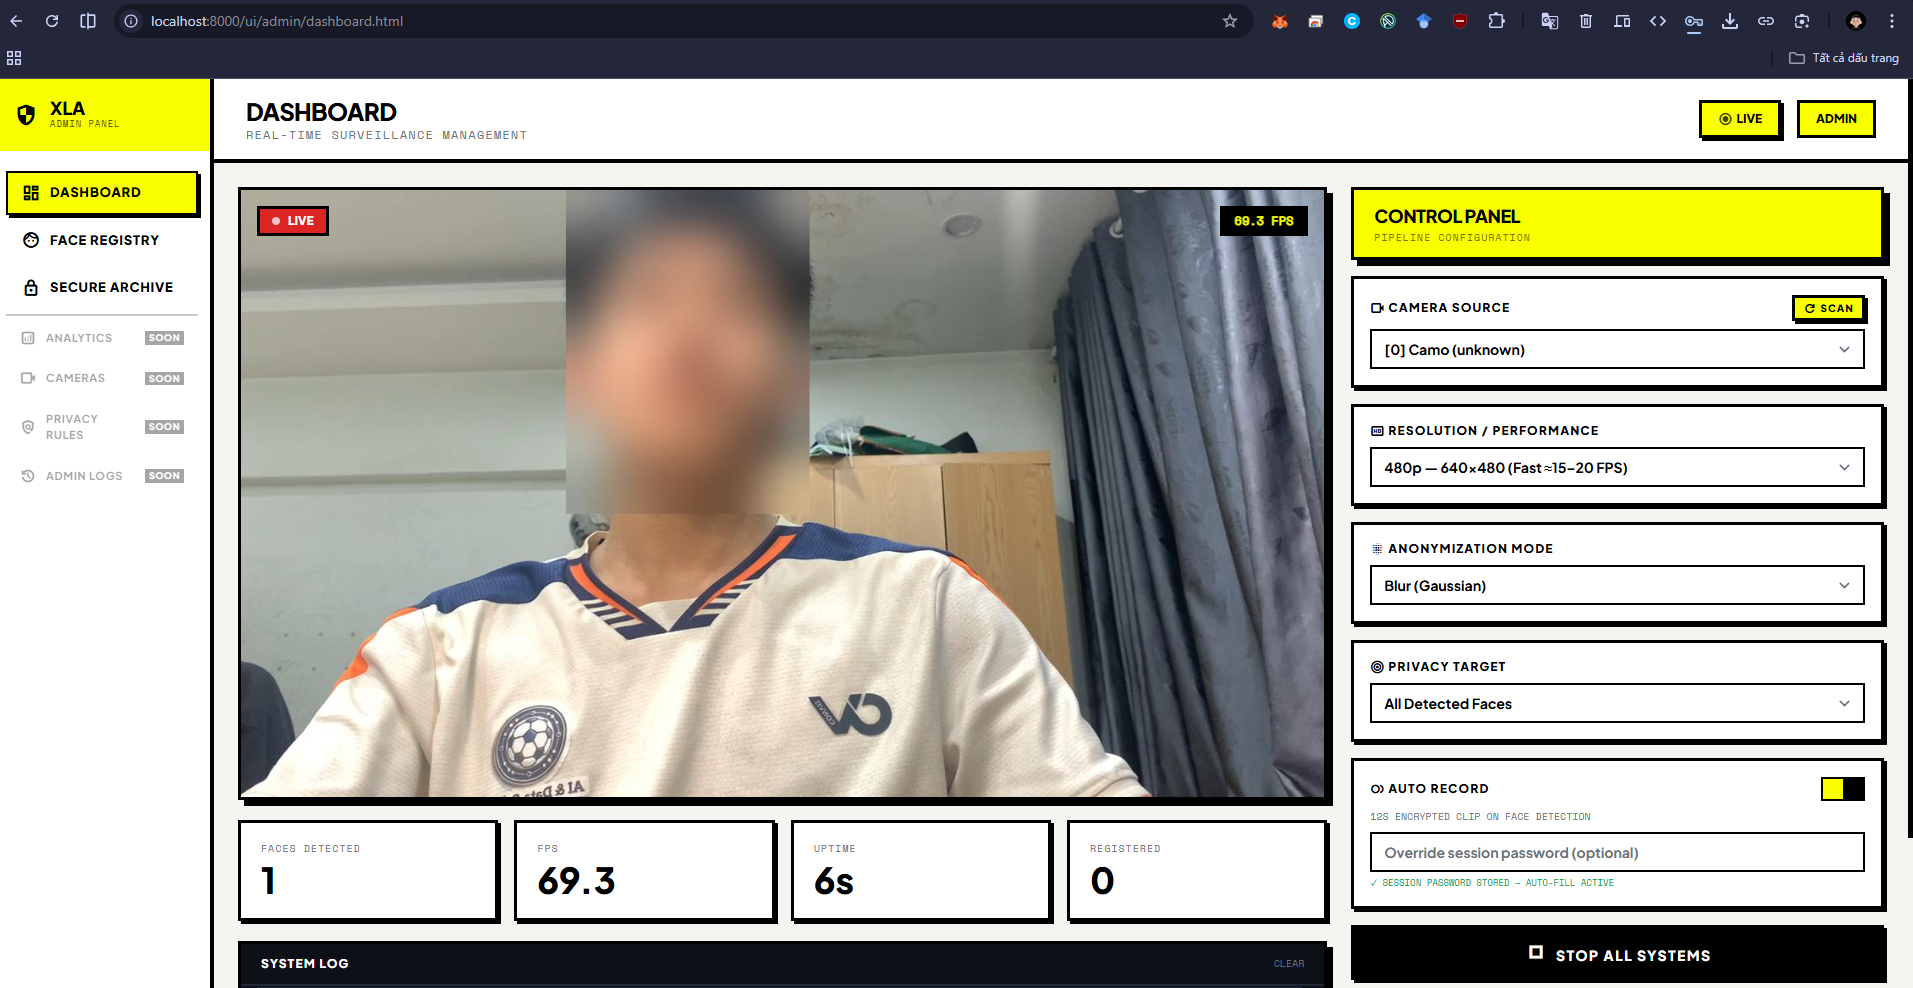
\includegraphics[width=0.30\textwidth]{blur.png} &
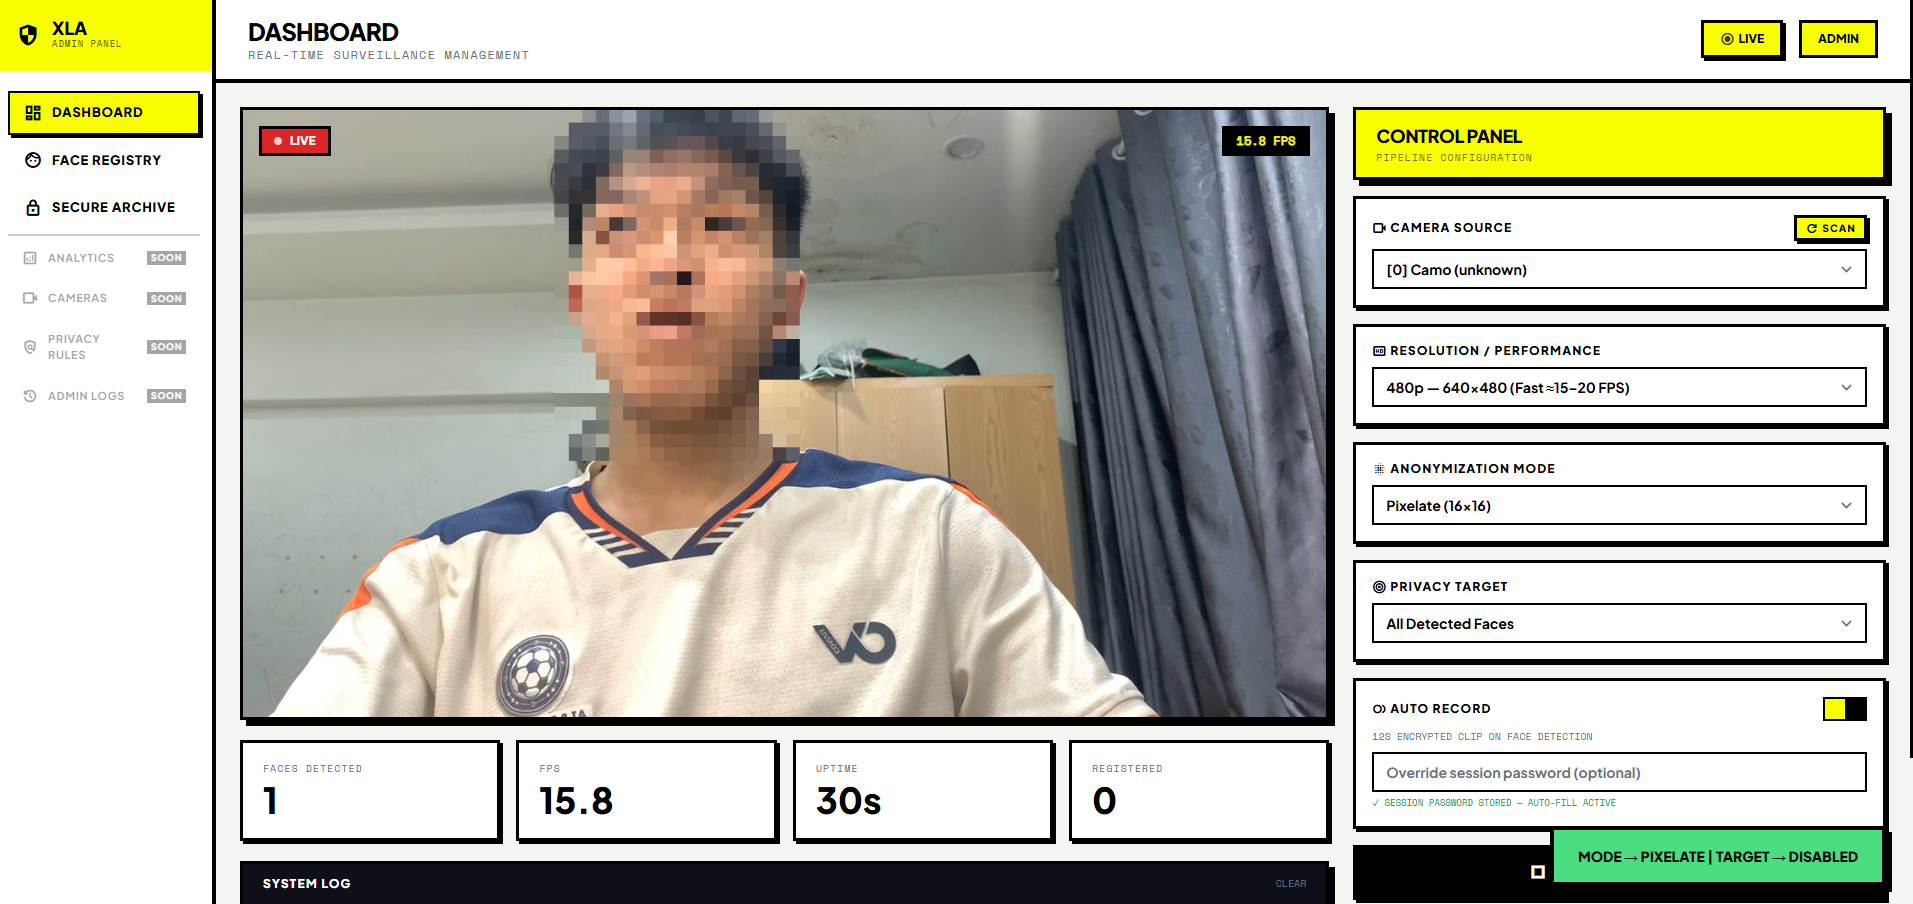
\includegraphics[width=0.30\textwidth]{pixelate.png} &
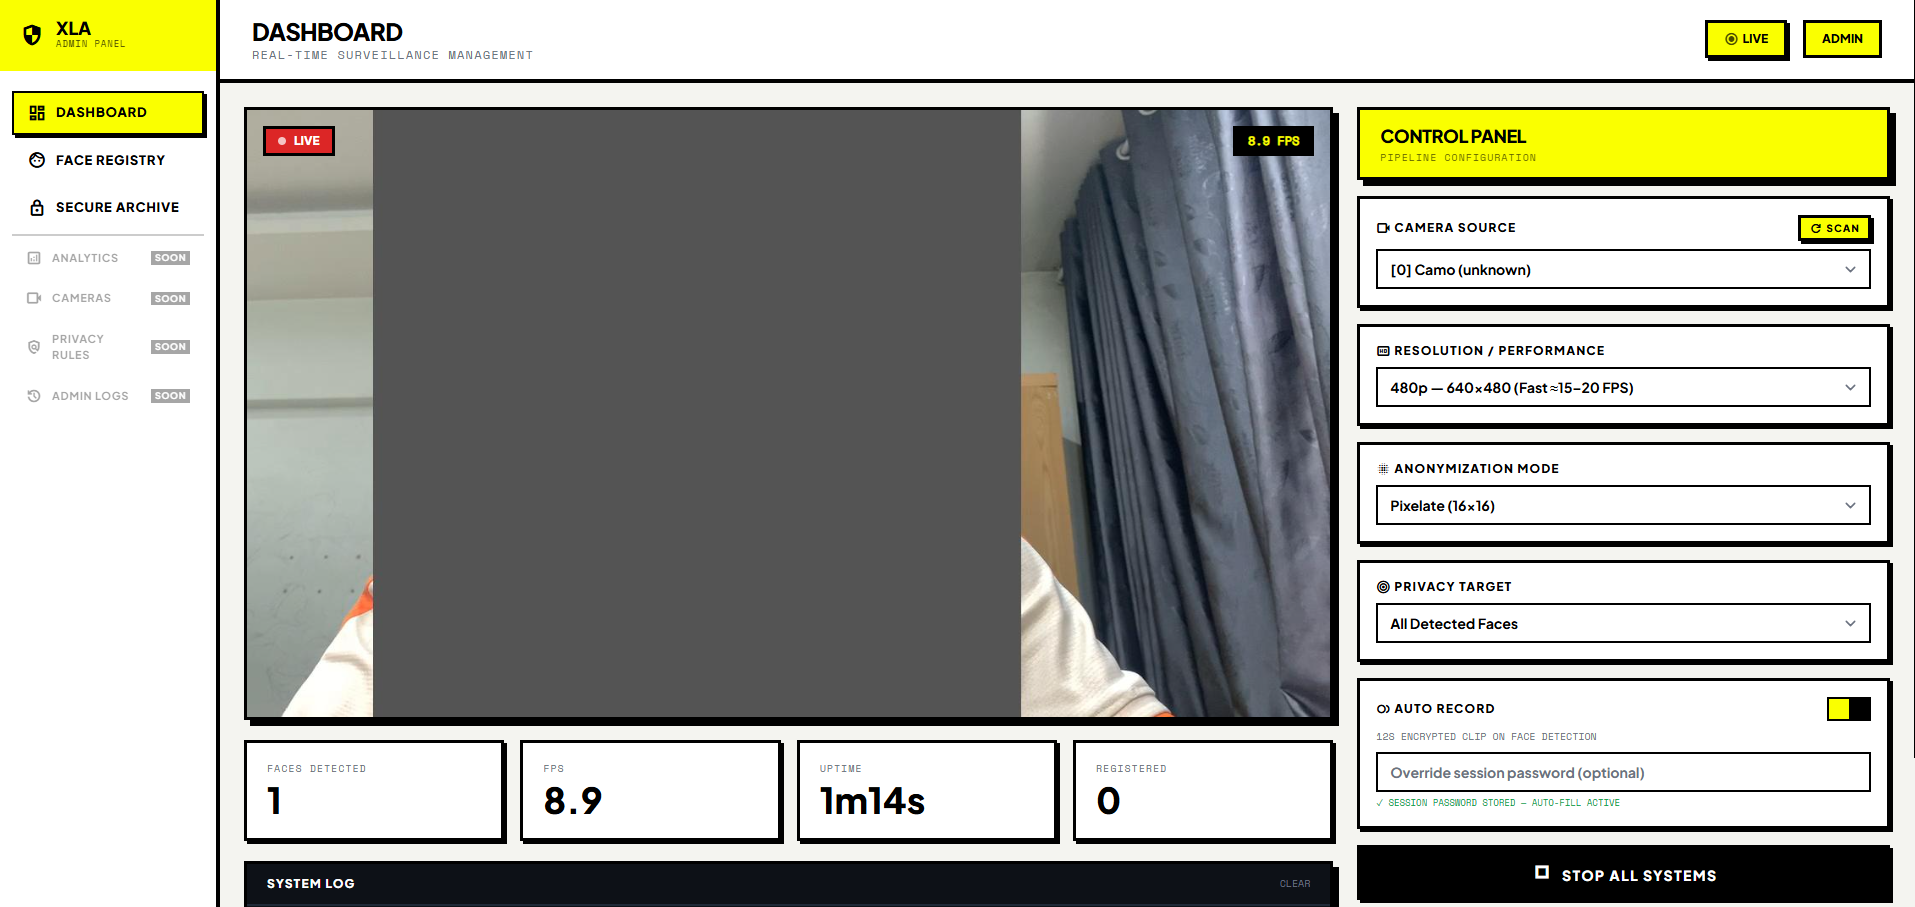
\includegraphics[width=0.30\textwidth]{headcloak.png} \\[1pt]
{\footnotesize\textbf{blur}} {\footnotesize\textit{--- Gaussian nhẹ}} &
{\footnotesize\textbf{pixelate}} {\footnotesize\textit{--- Mosaic}} &
{\footnotesize\textbf{headcloak}} {\footnotesize\textit{--- Mix+Noise}} \\[4pt]
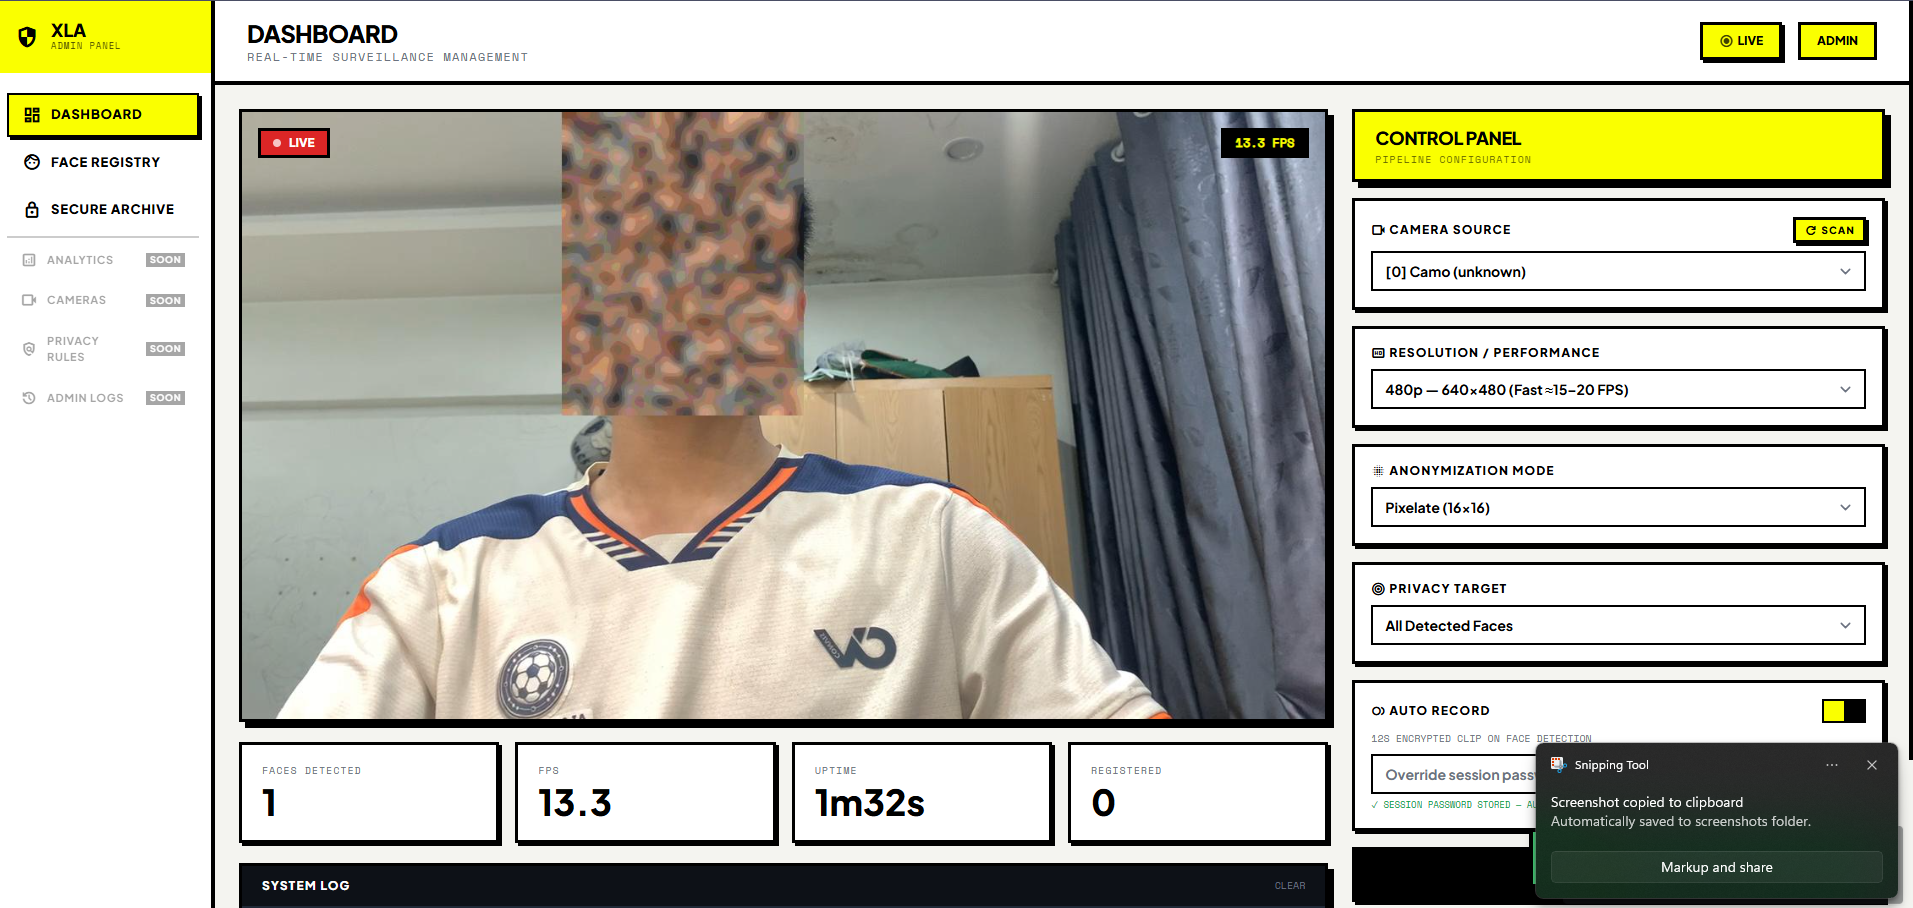
\includegraphics[width=0.30\textwidth]{obliterate.png} &
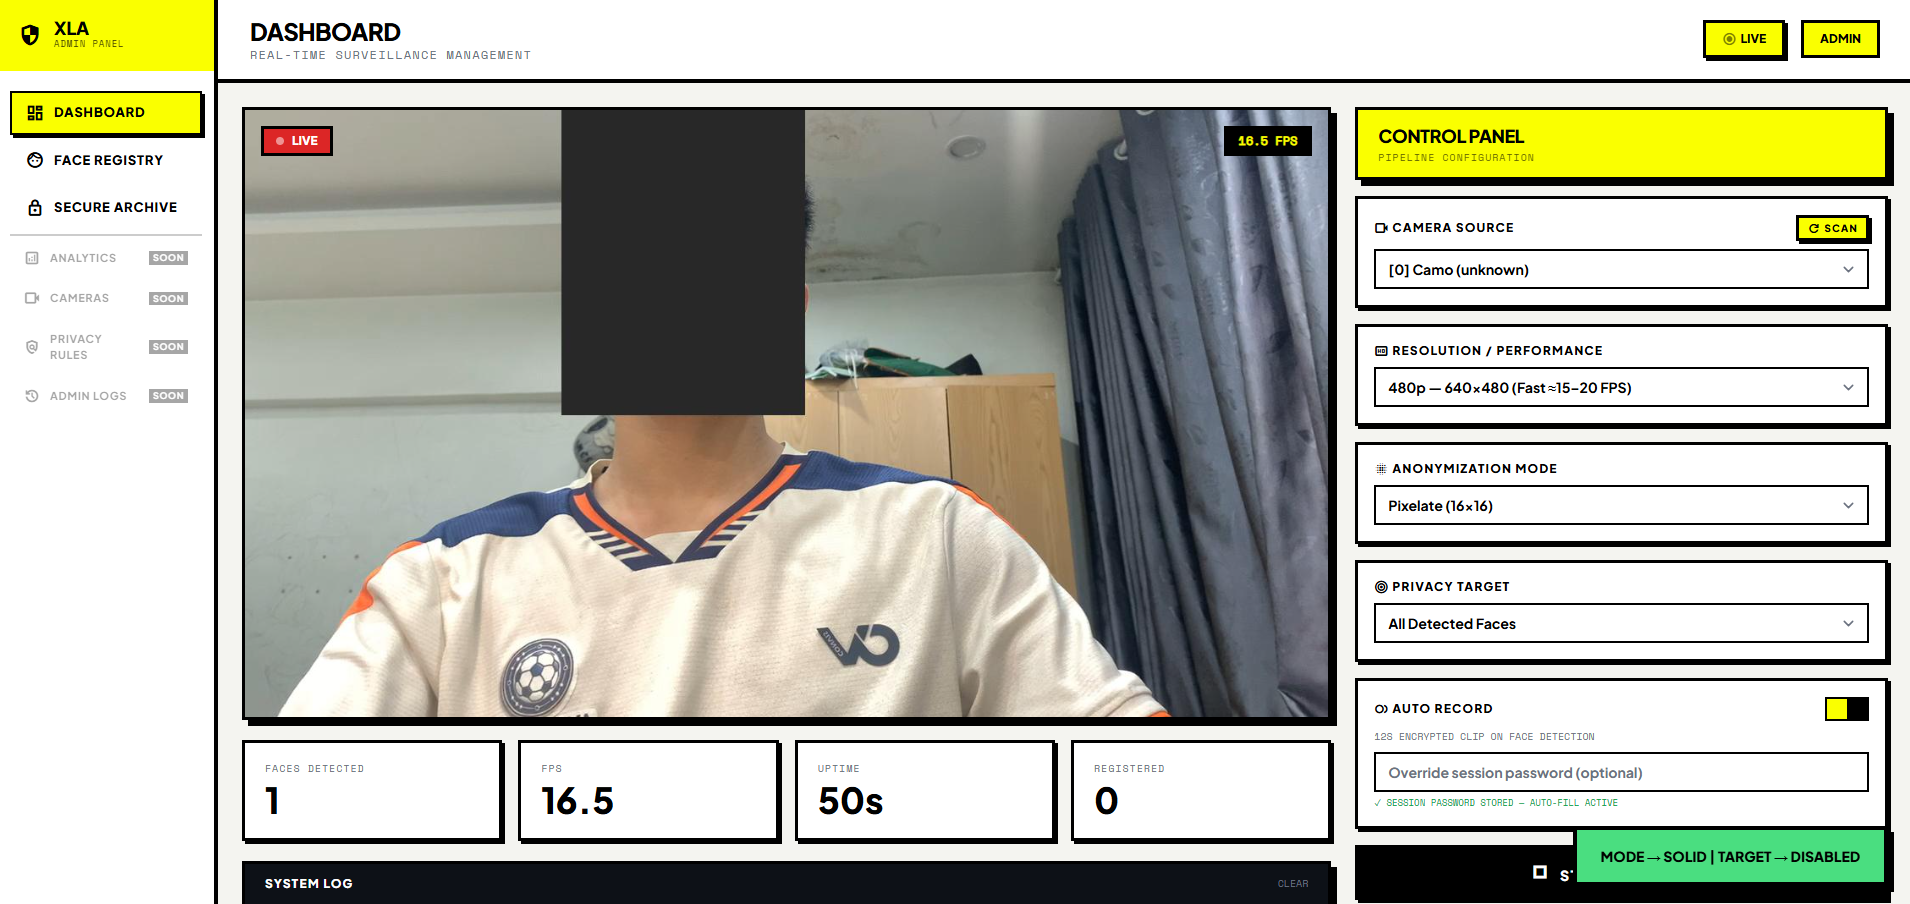
\includegraphics[width=0.30\textwidth]{solid.png} &
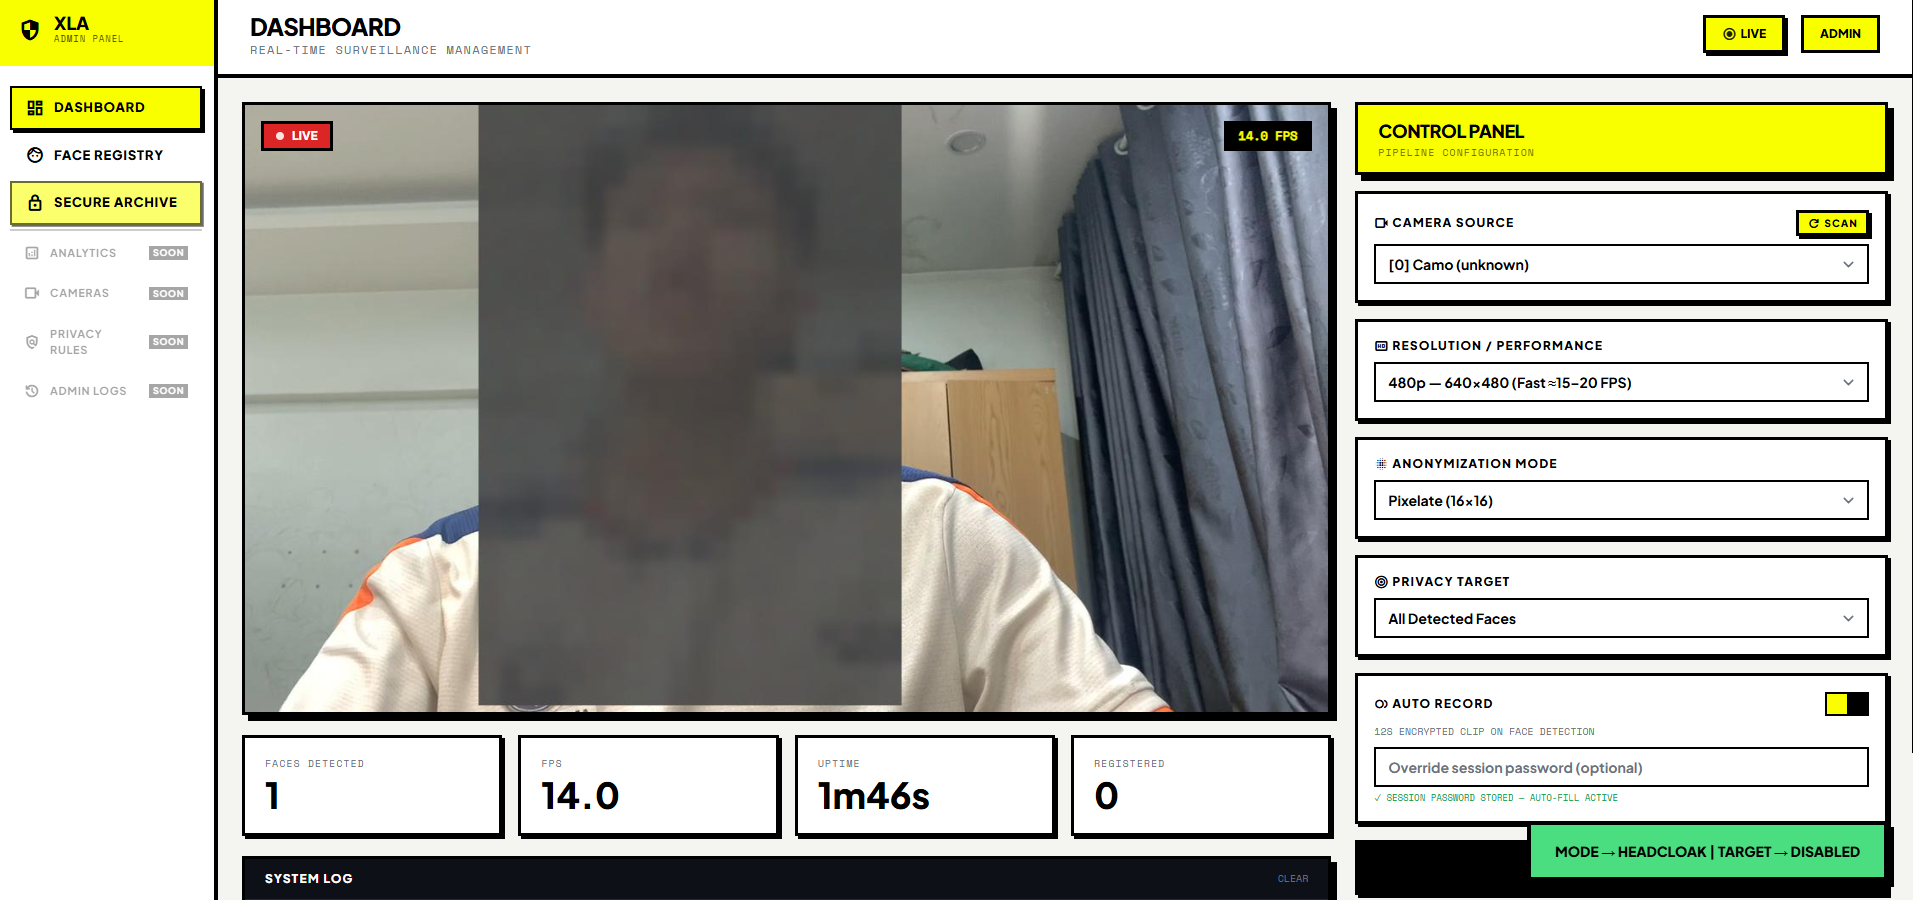
\includegraphics[width=0.30\textwidth]{silhouette.png} \\[1pt]
{\footnotesize\textbf{obliterate}} {\footnotesize\textit{--- 4-step}} &
{\footnotesize\textbf{solid}} {\footnotesize\textit{--- Black box}} &
{\footnotesize\textbf{silhouette}} {\footnotesize\textit{--- Extreme}} \\
\end{tabular}
\end{center}
\end{frame}

% ---- FRAME 9: Chi tiết modes ----
\begin{frame}[fragile]{Chi Tiết Các Chế Độ \& Kỹ Thuật Obliterate}
\begin{columns}[T]
\column{0.50\textwidth}
\begin{tabular}{llll}
\toprule
\textbf{Mode} & \textbf{Kỹ thuật} & \textbf{CPU} & \textbf{FPS*} \\
\midrule
\texttt{blur}       & Gaussian downscale & Thấp    & $\sim$25 \\
\texttt{pixelate}   & Bilinear+Nearest   & Rất thấp & $\sim$28 \\
\texttt{solid}      & Constant fill      & Tối thiểu & $\sim$30 \\
\texttt{headcloak}  & Mix+Noise+GBlur    & TB      & $\sim$18 \\
\texttt{obliterate} & 4-step pipeline    & Cao     & $\sim$12 \\
\texttt{silhouette} & Extreme cloak      & Rất cao & $\sim$8  \\
\bottomrule
\multicolumn{4}{l}{\scriptsize *CPU mid-range, proc\_width=640}
\end{tabular}
\vspace{0.3em}
\begin{block}{\faExpand\ Expand Box --- headcloak}
\footnotesize
Mở rộng vùng blur trước khi áp dụng:\\
Left/Right: $\pm35$--$70\%$ \ \ Top: $+70$--$120\%$ \ \ Bottom: $+25$--$50\%$\\
$\Rightarrow$ Che cả tóc, tai, jawline
\end{block}
\column{0.46\textwidth}
\begin{lstlisting}[language=Python,
  caption={privacy.py --- obliterate}]
def _obliterate_features(roi,...):
  """4-step, IRREVERSIBLE"""
  h, w = roi.shape[:2]

  # 1. Compress to 8% - destroy detail
  small = cv2.resize(roi,
    (int(w*0.08), int(h*0.08)),
    interpolation=INTER_AREA)
  work = cv2.resize(small, (w,h),
    interpolation=INTER_NEAREST)

  # 2. Scramble 12x12 blocks
  work = _scramble_blocks(
    work, block_size=12, seed=1337)

  # 3. Heavy Gaussian blur
  work = cv2.GaussianBlur(
    work, (35,35), 0)

  # 4. Quantize to 10 colors
  work = _quantize_colors(
    work, levels=10)
  return work
\end{lstlisting}
\end{columns}
\end{frame}

% ================================================================
\section{Backend \& Pipeline}
% ================================================================

% ---- FRAME 10: FastAPI ----
\begin{frame}{FastAPI Backend --- REST + WebSocket + Hot-reload}
\begin{columns}[T]
\column{0.50\textwidth}
\begin{block}{\faServer\ Các nhóm Endpoint}
\footnotesize\renewcommand{\arraystretch}{1.2}
\begin{tabular}{ll}
\texttt{GET /health}            & Server status \\
\texttt{GET /presets}           & 4 config presets \\
\hline
\texttt{POST /anonymize}        & Blur ảnh upload \\
\texttt{POST /pipeline/start}   & Start live pipeline \\
\texttt{PATCH /pipeline/config} & \textbf{Hot-reload} config \\
\hline
\texttt{GET /stream/mjpeg}      & MJPEG video stream \\
\texttt{WS /stream/ws}          & WebSocket binary \\
\hline
\texttt{GET/POST /members}      & Quản lý thành viên \\
\texttt{GET /clips}             & List clip đã ghi \\
\texttt{POST /clips/decrypt}    & Admin decrypt clip \\
\end{tabular}
\end{block}
\column{0.46\textwidth}
\begin{block}{\faDatabase\ 4 Preset Cấu Hình}
\footnotesize\renewcommand{\arraystretch}{1.3}
\begin{tabular}{lll}
\textbf{Preset} & \textbf{Mode} & \textbf{YOLO} \\
\hline
\texttt{fast}     & pixelate   & 416 px \\
\texttt{balanced} & headcloak  & 512 px \\
\texttt{strong}   & obliterate & 512 px \\
\texttt{strict}   & headcloak  & 416 px \\
\end{tabular}
\end{block}
\begin{block}{\faBolt\ Hot-reload + Streaming}
\footnotesize
\textbf{Hot-reload:} \texttt{PATCH /pipeline/config}\\
Đổi mode, threshold, proc\_width \textbf{không restart} server\\[3pt]
\textbf{Streaming:} MJPEG (\texttt{<img>}) hoặc\\
WebSocket (binary, low-latency)
\end{block}
\end{columns}
\end{frame}

% ---- FRAME 11: Live Pipeline ----
\begin{frame}{Live Pipeline --- Luồng Xử Lý Real-time}
\begin{center}
\begin{tikzpicture}[node distance=0.45cm and 0.65cm,
    scale=0.76, every node/.style={scale=0.76}]
  \node[module, minimum width=1.9cm] (cam) {\faCamera\\Camera};
  \node[module, right=of cam, minimum width=2.1cm] (fr)
    {Frame\\Reader\\Thread};
  \node[module, right=of fr, minimum width=2.1cm] (yolo)
    {YOLOv11\\detect\\\_every=2};
  \node[module, right=of yolo, minimum width=2.1cm] (smooth)
    {BBox\\Smoother\\EMA $\alpha$=0.7};
  \node[module, right=of smooth, minimum width=2.1cm] (iface)
    {InsightFace\\buffalo\_l\\512-dim};

  \node[module, below=1.3cm of yolo, xshift=1.1cm, minimum width=2.2cm] (db)
    {FamilyDB\\match()\\cosine};
  \node[greenmod, left=0.65cm of db, minimum width=2.2cm] (anon)
    {anonymize\\\_faces()\\7 modes};
  \node[highlight, right=0.65cm of db, minimum width=2.2cm] (rec)
    {ClipRecorder\\AES-256\\GCM};

  \draw[arrow] (cam) -- (fr);
  \draw[arrow] (fr)  -- (yolo);
  \draw[arrow] (yolo) -- (smooth);
  \draw[arrow] (smooth) -- (iface);
  \draw[arrow] (iface) -- ++(0,-0.85) -| (db);
  \draw[arrow] (db) -- (anon);
  \draw[arrow] (db) -- (rec);
  \draw[->,dashed,gray,>=Stealth] (anon) -- ++(-2.5,0)
    node[left,font=\tiny]{MJPEG/WS};
  \draw[->,dashed,accent,>=Stealth,thick] (rec) -- ++(2.1,0)
    node[right,font=\tiny\color{accent}]{.enc + .mp4};
\end{tikzpicture}
\end{center}
\vspace{-0.2em}
\begin{columns}[T]
\column{0.32\textwidth}
\begin{block}{\faCogs\ FrameReader Thread}
\footnotesize
\texttt{cv2.VideoCapture.read()} là blocking.\\
Thread riêng $\Rightarrow$ frame luôn fresh,\\
không bị stale khi YOLO chạy.
\end{block}
\column{0.32\textwidth}
\begin{block}{\faCogs\ BBox Smoother}
\footnotesize
EMA: $\hat{b}_t = \alpha b_t + (1-\alpha)\hat{b}_{t-1}$\\
$\alpha=0.7$ — responsive + mượt.\\
Loại bỏ jitter frame-by-frame.
\end{block}
\column{0.32\textwidth}
\begin{block}{\faBell\ detect\_every=2}
\footnotesize
YOLO chạy 1 lần / 2 frame.\\
Frame bỏ qua dùng lại bbox cũ.\\
$\Rightarrow$ Giảm 50\% compute cost.
\end{block}
\end{columns}
\end{frame}

% ================================================================
\section{Bảo Mật}
% ================================================================

% ---- FRAME 12: AES-256-GCM ----
\begin{frame}{AES-256-GCM --- Mã Hoá Video Gốc}
\begin{columns}[T]
\column{0.50\textwidth}
\begin{center}
\begin{tikzpicture}[node distance=0.5cm and 0.8cm,
    scale=0.78, every node/.style={scale=0.78}]
  \node[module, minimum width=2.6cm] (frame) {Raw Frames\\từ camera};
  \node[module, right=0.7cm of frame, minimum width=2.6cm] (pack)
    {\_pack\_frames()\\JPEG 90\%};
  \node[highlight, right=0.7cm of pack, minimum width=2.6cm] (aes)
    {AES-256-GCM\\encrypt()};

  \node[module, below=1cm of frame, minimum width=2.6cm] (salt)
    {secrets.token\_bytes(32)\\Per-clip Salt};
  \node[module, below=1cm of pack, minimum width=2.6cm] (pbkdf2)
    {PBKDF2-SHA256\\390\,000 rounds};
  \node[highlight, right=0.7cm of aes, minimum width=2.8cm] (enc)
    {.enc file\\{\tiny[32B salt][12B nonce]}\\{\tiny ciphertext+GCM tag}};

  \draw[arrow] (frame) -- (pack);
  \draw[arrow] (pack)  -- (aes);
  \draw[arrow] (salt)  -- (pbkdf2);
  \draw[arrow] (pbkdf2) -- (aes) node[midway,right,font=\tiny]{32B key};
  \draw[arrow] (aes) -- (enc);
  \node[font=\tiny,below=0.05cm of salt]{password admin};
\end{tikzpicture}
\end{center}
\column{0.46\textwidth}
\begin{block}{\faKey\ Per-clip Salt}
\footnotesize
Mỗi clip = 1 salt 32B ngẫu nhiên.\\
Cùng password $\Rightarrow$ \textbf{khác key}.\\
Lộ 1 clip $\neq$ lộ toàn bộ.
\end{block}
\begin{block}{\faLock\ AES-256-GCM}
\footnotesize
\textbf{Authenticated Encryption.}\\
Auth Tag 128-bit tích hợp.\\
Sửa 1 bit $\Rightarrow$ decrypt fail ngay.
\end{block}
\begin{block}{\faClock\ PBKDF2-SHA256}
\footnotesize
390\,000 rounds (OWASP 2023).\\
Brute-force 8 ký tự:\\
$\approx$ \textbf{hàng trăm nghìn năm}.
\end{block}
\end{columns}
\end{frame}

% ---- FRAME 13: Admin Auth ----
\begin{frame}[fragile]{Admin Authentication --- PBKDF2 + Timing-safe}
\begin{columns}[T]
\column{0.52\textwidth}
\begin{lstlisting}[language=Python,
  caption={admin\_auth.py}]
_ITERATIONS = 390_000  # OWASP 2023

def _pbkdf2(password, salt,
            iters=_ITERATIONS):
    kdf = PBKDF2HMAC(
        algorithm=hashes.SHA256(),
        length=32,   # 256-bit key
        salt=salt,
        iterations=iters,
    )
    return kdf.derive(
        password.encode("utf-8"))

def _ct_equal(a: bytes, b: bytes):
    """Chong Timing Attack."""
    # '==' dung o byte sai dau tien
    # -> attacker do thoi gian -> guess
    # hmac.compare_digest: CONSTANT TIME
    return hmac.compare_digest(a, b)
\end{lstlisting}
\column{0.44\textwidth}
\begin{block}{\faDatabase\ Credentials File}
\footnotesize
\begin{lstlisting}[numbers=none]
{
  "salt": "aGVsbG8h...",
  "hash": "c2VjcmV0...",
  "iterations": 390000
}
\end{lstlisting}
\textbf{Không lưu plaintext password.}\\
Ngay cả developer không biết.
\end{block}
\begin{alertblock}{\faExclamationTriangle\ Timing Attack}
\footnotesize
\texttt{a == b} dừng ở byte sai đầu\\
$\Rightarrow$ thời gian response khác nhau\\
$\Rightarrow$ hacker đoán được từng byte\\[3pt]
\texttt{hmac.compare\_digest}: luôn chạy hết\\
$\Rightarrow$ constant-time, không leak
\end{alertblock}
\end{columns}
\end{frame}

% ================================================================
\section{Demo \& Kết Quả}
% ================================================================

% ---- FRAME 14: Admin Dashboard ----
\begin{frame}{Giao Diện Admin Dashboard}
\begin{columns}[T]
\column{0.62\textwidth}
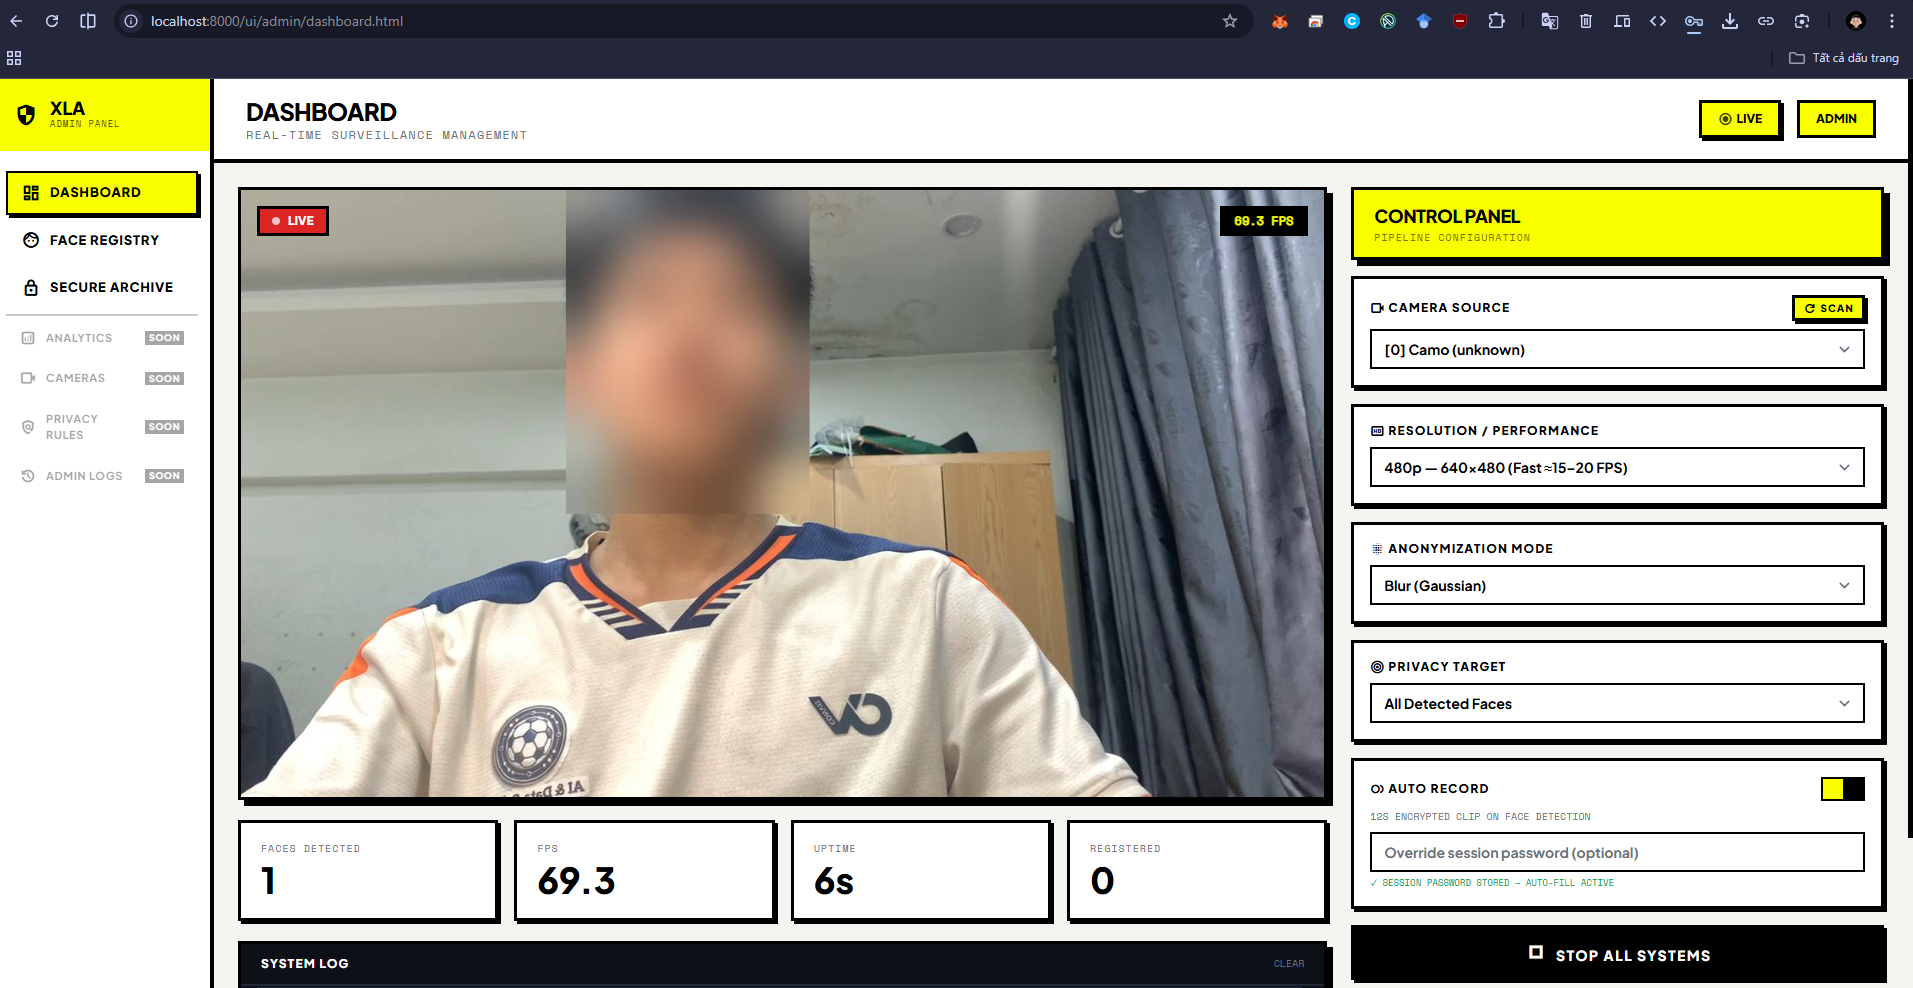
\includegraphics[width=\linewidth]{admin_dashboard.png}
\column{0.34\textwidth}
\begin{block}{\faDesktop\ Admin Dashboard}
\footnotesize
URL: \texttt{/admin/dashboard.html}
\begin{itemize}
  \item Xem live stream đã xử lý
  \item Điều khiển pipeline (Start/Stop)
  \item Đổi chế độ ẩn danh on-the-fly
  \item Xem FPS, latency realtime
  \item Quản lý thành viên gia đình
\end{itemize}
\end{block}
\begin{alertblock}{\faLock\ Yêu cầu đăng nhập}
\footnotesize
Chỉ Admin mới truy cập được.\\
Guest $\Rightarrow$ redirect đăng nhập.
\end{alertblock}
\end{columns}
\end{frame}

% ---- FRAME 15: User Portal ----
\begin{frame}{Giao Diện User Portal}
\begin{columns}[T]
\column{0.62\textwidth}
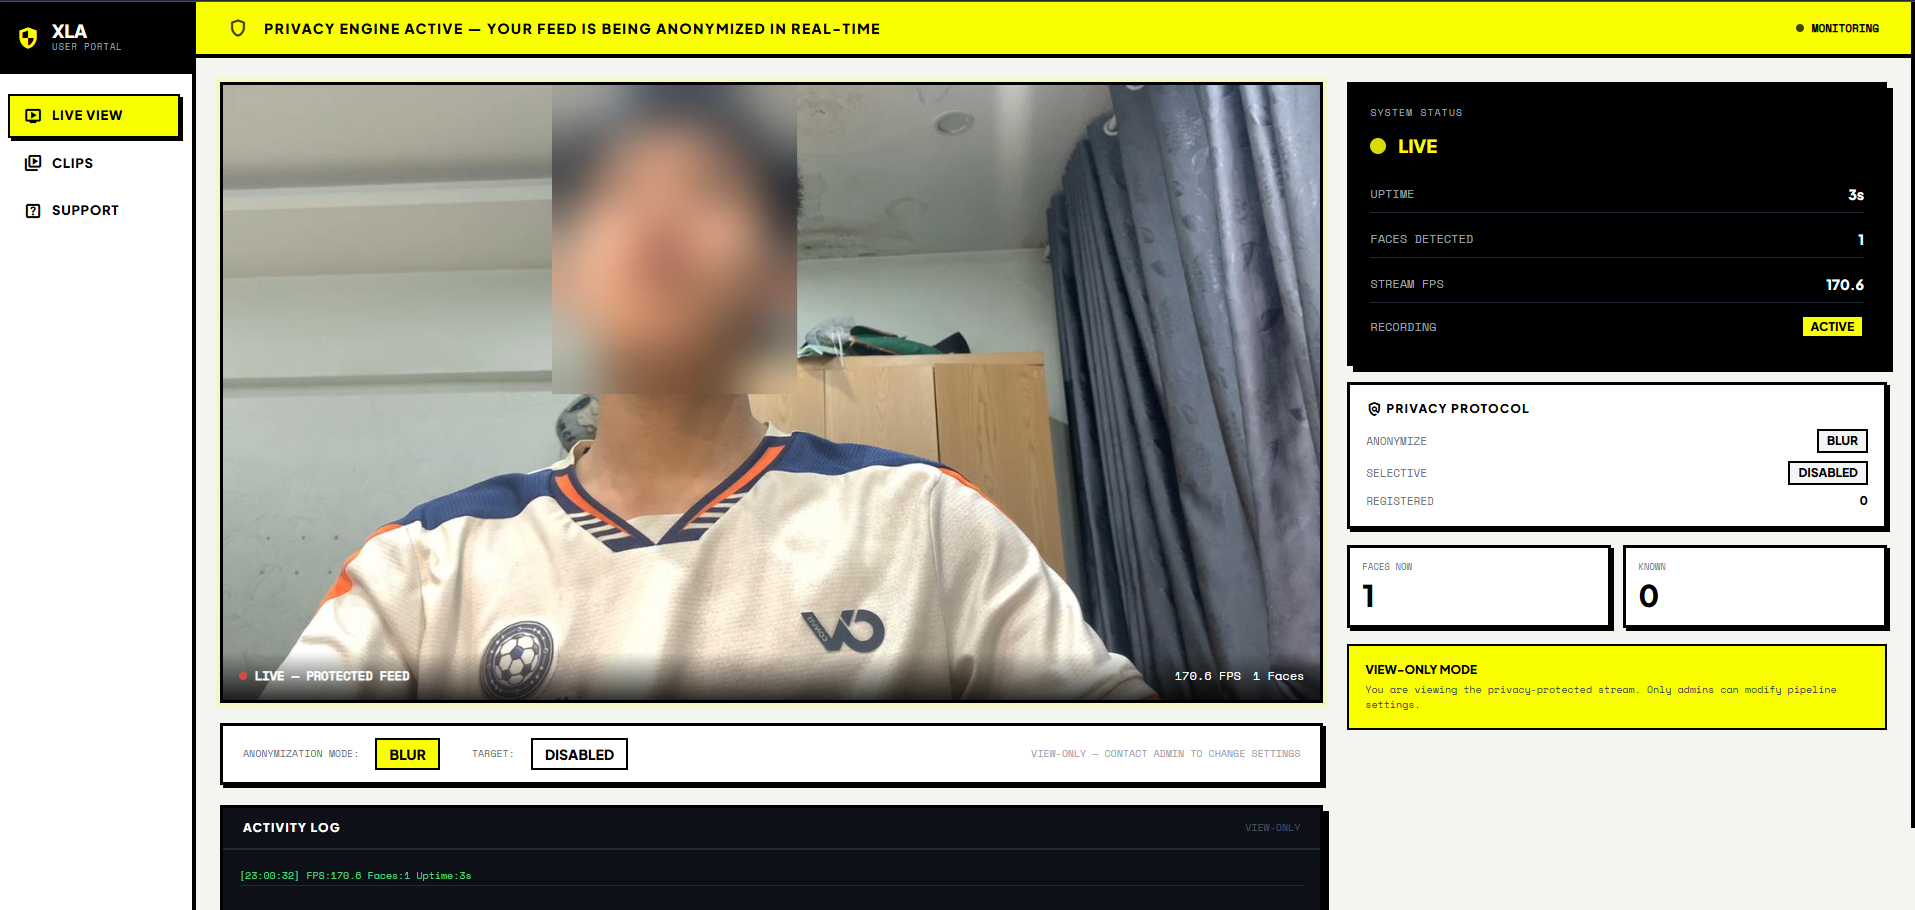
\includegraphics[width=\linewidth]{user_portal.png}
\column{0.34\textwidth}
\begin{block}{\faEye\ User Portal}
\footnotesize
URL: \texttt{/user/live-portal.html}
\begin{itemize}
  \item Xem stream đã \textbf{ẩn danh hoá}
  \item \textbf{Không cần đăng nhập}
  \item Khuôn mặt người lạ đã bị che
  \item Thành viên: hiển thị tên
\end{itemize}
\end{block}
\begin{block}{\faUsers\ Phân quyền}
\footnotesize
\begin{tabular}{ll}
\textbf{Role} & \textbf{Quyền truy cập} \\
\hline
Admin & Full control \\
User  & View only \\
Guest & Public stream \\
\end{tabular}
\end{block}
\end{columns}
\end{frame}

% ---- FRAME 16: Benchmark ----
\begin{frame}{Kết Quả Benchmark --- FPS Theo Chế Độ}
\begin{columns}[T]
\column{0.52\textwidth}
\begin{block}{\faChartBar\ FPS đo trên CPU mid-range}
\footnotesize\renewcommand{\arraystretch}{1.35}
\begin{tabular}{lrrl}
\textbf{Mode} & \textbf{FPS} & \textbf{CPU} & \textbf{Dải màu FPS} \\
\hline
blur        & 69.3 & Thấp    & \textcolor{blue!70}{\rule{5.5cm}{3pt}} \\
pixelate    & 15.8 & Rất thấp & \textcolor{teal!70}{\rule{1.2cm}{3pt}} \\
solid       & 16.5 & Tối thiểu & \textcolor{teal!50}{\rule{1.3cm}{3pt}} \\
headcloak   & 14.0 & Trung bình & \textcolor{orange!70}{\rule{1.1cm}{3pt}} \\
obliterate  & 13.3 & Cao     & \textcolor{orange!90}{\rule{1.05cm}{3pt}} \\
silhouette  &  8.9 & Rất cao & \textcolor{red!70}{\rule{0.7cm}{3pt}} \\
\end{tabular}
\end{block}
\column{0.44\textwidth}
\begin{block}{\cmark\ Nhận xét}
\begin{itemize}\footnotesize
  \item \texttt{blur}: \textbf{69 FPS} --- cực kỳ nhẹ
  \item \texttt{pixelate/solid}: $\sim$16 FPS
  \item \texttt{headcloak}: $\sim$14 FPS --- mặc định
  \item \texttt{obliterate}: $\sim$13 FPS --- rất mạnh
  \item \texttt{silhouette}: $\sim$9 FPS --- cực mạnh
  \item Tất cả chạy trên \textbf{CPU} (không GPU)
\end{itemize}
\end{block}
\begin{block}{\cmark\ Nhận diện}
\begin{itemize}\footnotesize
  \item 2 thành viên đăng ký: \textbf{đúng 100\%}
  \item Threshold 0.35 + 100 mẫu: ổn định
  \item Khánh (chưa đăng ký): bị blur đúng
\end{itemize}
\end{block}
\end{columns}
\end{frame}

% ---- FRAME 17: Kết quả ----
\begin{frame}{Kết Quả Đạt Được}
\begin{columns}[T]
\column{0.48\textwidth}
\begin{block}{\cmark\ Privacy --- Đạt}
\begin{itemize}\footnotesize
  \item 7 chế độ ẩn danh từ nhẹ đến cực mạnh
  \item Người lạ: ẩn danh hoàn toàn
  \item Thành viên đăng ký: không bị che
  \item Hot-reload mode không cần restart
\end{itemize}
\end{block}
\begin{block}{\cmark\ Security --- Đạt}
\begin{itemize}\footnotesize
  \item AES-256-GCM: mã hoá + authenticated
  \item PBKDF2-SHA256 390\,000 iter (OWASP)
  \item Per-clip salt: không reuse key
  \item Constant-time compare: no timing leak
\end{itemize}
\end{block}
\column{0.48\textwidth}
\begin{block}{\cmark\ Detection \& Recognition --- Khoa}
\begin{itemize}\footnotesize
  \item YOLOv11n-face: nhẹ, nhanh, chính xác
  \item InsightFace buffalo\_l: 512-dim embedding
  \item Vectorized batch matching O(n)
  \item BBox EMA smoother: loại bỏ jitter
\end{itemize}
\end{block}
\begin{block}{\cmark\ Backend \& UI --- Khánh}
\begin{itemize}\footnotesize
  \item FastAPI REST + WebSocket + SSE
  \item MJPEG + WebSocket dual streaming
  \item 4 preset cấu hình sẵn sàng dùng
  \item 6 trang HTML, phân quyền Admin/User
\end{itemize}
\end{block}
\end{columns}
\end{frame}

% ---- FRAME 18: Hạn chế & Q&A ----
\begin{frame}{Hạn Chế \& Câu Hỏi Thường Gặp}
\begin{columns}[T]
\column{0.46\textwidth}
\begin{alertblock}{\faTimes\ Hạn chế hiện tại}
\begin{itemize}\footnotesize
  \item CPU-only --- FPS bị giới hạn
  \item Chỉ 2 thành viên được đăng ký
  \item Chưa có audit log
  \item Chưa data retention policy
\end{itemize}
\end{alertblock}
\begin{block}{\faArrowRight\ Hướng mở rộng}
\begin{itemize}\footnotesize
  \item GPU inference (CUDA / TensorRT)
  \item Nhiều camera đồng thời
  \item Key Escrow / Shamir Secret Sharing
  \item Compliance dashboard + audit log
\end{itemize}
\end{block}
\column{0.50\textwidth}
\begin{block}{\faQuestionCircle\ Câu hỏi thường gặp}
\footnotesize\renewcommand{\arraystretch}{1.5}
\begin{tabularx}{\linewidth}{lX}
\textbf{Q: Quên password?} & Không recover được --- by design. Production: Key Escrow. \\
\hline
\textbf{Q: AES-GCM vs CBC?} & GCM = Authenticated. CBC chỉ encrypt, không verify integrity. \\
\hline
\textbf{Q: 390k iterations?} & OWASP 2023 minimum. Đủ chậm cho brute-force, đủ nhanh cho UX. \\
\hline
\textbf{Q: GDPR?} & Privacy by Design Art.25. Cần thêm: audit log, consent, retention. \\
\end{tabularx}
\end{block}
\end{columns}
\end{frame}

% ---- FRAME 19: Final ----
\begin{frame}[plain]
\begin{tikzpicture}[remember picture, overlay]
  \fill[primary] (current page.north west)
    rectangle ([yshift=-0.48\paperheight] current page.north east);
  \node[text=white, font=\LARGE\bfseries, anchor=center]
    at ([yshift=-1.8cm] current page.north)
    {Cảm ơn Thầy/Cô đã lắng nghe!};
  \node[text=white!80, font=\large, anchor=center]
    at ([yshift=-2.9cm] current page.north)
    {XLA Face Privacy System};
  \node[text=white!60, font=\normalsize, anchor=center]
    at ([yshift=-3.7cm] current page.north)
    {Privacy by Default \textbullet\ Evidence on Demand \textbullet\ AES-256-GCM};
\end{tikzpicture}

\vspace{4.8cm}
\begin{columns}[c]
\column{0.56\textwidth}
\begin{block}{\faUsers\ Nhóm thực hiện}
\footnotesize\renewcommand{\arraystretch}{1.5}
\begin{tabular}{lll}
\textcolor{accent}{\textbf{Đạt}} & Leader & AES-256-GCM · PBKDF2 · Blur \\
\textbf{Khánh} & Backend & FastAPI · Pipeline · Streaming \\
\textbf{Khoa} & Detection & YOLOv11 · InsightFace · DB \\
\end{tabular}
\end{block}
\column{0.38\textwidth}
\begin{block}{\faCode\ Repository}
\footnotesize
\faGithub\ \texttt{Poicitaco/XLA\_T3}\\
Branch: \texttt{feature/cipher}\\
\faServer\ Port \texttt{8000} · \faPython\ Python 3.13
\end{block}
\end{columns}
\vspace{0.4em}
\begin{center}
\large\textbf{\textcolor{primary}{Sẵn sàng trả lời câu hỏi!}}
\end{center}
\end{frame}

\end{document}


% ---- Theme ----
\usetheme{Madrid}
\usecolortheme{whale}
\usefonttheme{professionalfonts}
\setbeamertemplate{navigation symbols}{}
\setbeamertemplate{footline}[frame number]

% ---- Màu sắc ----
\definecolor{primary}{RGB}{0,51,102}
\definecolor{accent}{RGB}{220,50,47}
\definecolor{secbg}{RGB}{230,240,255}
\definecolor{codebg}{RGB}{248,248,248}
\definecolor{darkgreen}{RGB}{0,100,50}
\definecolor{gold}{RGB}{180,130,0}

\setbeamercolor{palette primary}{bg=primary, fg=white}
\setbeamercolor{palette secondary}{bg=primary!80, fg=white}
\setbeamercolor{palette tertiary}{bg=primary!60, fg=white}
\setbeamercolor{frametitle}{bg=primary, fg=white}
\setbeamercolor{title}{fg=white}
\setbeamercolor{block title}{bg=primary, fg=white}
\setbeamercolor{block body}{bg=secbg}
\setbeamercolor{alerted text}{fg=accent}

% ---- Encoding / Language ----
\usepackage[utf8]{inputenc}
\usepackage[T5]{fontenc}
\usepackage[vietnamese]{babel}

% ---- Packages ----
\usepackage{listings}
\usepackage{booktabs}
\usepackage{tabularx}
\usepackage{array}
\usepackage{tikz}
\usetikzlibrary{shapes.geometric, arrows.meta, positioning, fit, backgrounds}
\usepackage{tcolorbox}
\tcbuselibrary{skins}
\usepackage{fontawesome5}
\usepackage{graphicx}
\usepackage{amsmath}
\usepackage{pifont}
\usepackage{subcaption}

\graphicspath{{./img/}{./image/}}

\newcommand{\cmark}{\textcolor{darkgreen}{\ding{51}}}
\newcommand{\xmark}{\textcolor{accent}{\ding{55}}}
\newcommand{\filecode}[1]{\texttt{\textcolor{primary}{\small #1}}}

% ---- Code style ----
\lstset{
  basicstyle=\ttfamily\footnotesize,
  keywordstyle=\color{primary}\bfseries,
  commentstyle=\color{darkgreen}\itshape,
  stringstyle=\color{accent},
  numbers=left, numberstyle=\tiny\color{gray}, numbersep=5pt,
  frame=tb, breaklines=true, showstringspaces=false,
  tabsize=2, backgroundcolor=\color{codebg},
}

% ---- TikZ styles ----
\tikzset{
  module/.style={rectangle, rounded corners=4pt,
    draw=primary, fill=secbg, thick,
    minimum height=1cm, minimum width=2.8cm,
    text width=2.6cm, align=center, font=\small},
  arrow/.style={->, >=Stealth, thick, color=primary},
  highlight/.style={rectangle, rounded corners=4pt,
    draw=accent, fill=accent!10, thick,
    minimum height=1cm, minimum width=2.8cm,
    text width=2.6cm, align=center, font=\small\bfseries},
  greenmod/.style={rectangle, rounded corners=4pt,
    draw=darkgreen, fill=darkgreen!10, thick,
    minimum height=1cm, minimum width=2.8cm,
    text width=2.6cm, align=center, font=\small},
}

% ============================================================
\begin{document}
% ============================================================

% ================================================================
%  TRANG TiTLE
% ================================================================
\begin{frame}[plain]
\begin{tikzpicture}[remember picture, overlay]
  \fill[primary] (current page.north west)
    rectangle ([yshift=-0.44\paperheight] current page.north east);

  \node[text=white, anchor=north, font=\Large\bfseries]
    at ([yshift=-1.2cm] current page.north)
    {XLA Face Privacy System};

  \node[text=white!85, anchor=north, font=\normalsize]
    at ([yshift=-2.1cm] current page.north)
    {Hệ Thống Camera Bảo Vệ Quyền Riêng Tư Khuôn Mặt Theo Thời Gian Thực};

  \node[text=white!60, anchor=north, font=\small]
    at ([yshift=-2.9cm] current page.north)
    {\faGraduationCap\ Môn: Xử Lý Ảnh Số \quad\faUniversity\ ĐH Phenikaa};
\end{tikzpicture}

\vspace{3.6cm}
\begin{columns}[c]
\column{0.52\textwidth}
\begin{block}{\faUsers\ Nhóm thực hiện}
\footnotesize\renewcommand{\arraystretch}{1.5}
\begin{tabular}{lll}
\textbf{Vai trò}          & \textbf{Họ tên}              & \textbf{MSSV} \\
\hline
\textcolor{accent}{\textbf{Leader}} & \textcolor{accent}{\textbf{Hoàng Tiến Đạt}} & 23010864 \\
Backend & Nghiêm Xuân Khánh  & 23010598 \\
Detection & Nguyễn Hữu Đăng Khoa & 23010901 \\
\end{tabular}
\end{block}

\column{0.43\textwidth}
\begin{block}{\faInfo\ Thông tin}
\footnotesize
\begin{itemize}
  \item Ngôn ngữ: \textbf{Python 3.13}
  \item Framework: \textbf{FastAPI}
  \item Model: \textbf{YOLOv11n-face + InsightFace}
  \item Bảo mật: \textbf{AES-256-GCM}
  \item Lớp: \textbf{KHDL\&AI}
\end{itemize}
\end{block}
\end{columns}
\end{frame}

% ================================================================
%  AGENDA
% ================================================================
\begin{frame}{Nội Dung Thuyết Trình}
\begin{columns}[T]
\column{0.48\textwidth}
\begin{block}{\faList\ Phần 1 --- Tổng quan}
\begin{enumerate}\footnotesize
  \item Vấn đề \& Giải pháp
  \item Kiến trúc hệ thống
  \item Phân công nhiệm vụ
\end{enumerate}
\end{block}
\begin{block}{\faCog\ Phần 2 --- Kỹ thuật}
\begin{enumerate}\footnotesize\setcounter{enumi}{3}
  \item Phát hiện khuôn mặt (YOLOv11)
  \item Nhận diện thành viên (InsightFace)
  \item 6 chế độ ẩn danh hoá
  \item Backend \& Live Pipeline
\end{enumerate}
\end{block}

\column{0.48\textwidth}
\begin{block}{\faLock\ Phần 3 --- Bảo mật}
\begin{enumerate}\footnotesize\setcounter{enumi}{7}
  \item Mã hoá AES-256-GCM
  \item Admin authentication (PBKDF2)
\end{enumerate}
\end{block}
\begin{block}{\faDesktop\ Phần 4 --- Demo \& Kết quả}
\begin{enumerate}\footnotesize\setcounter{enumi}{9}
  \item Giao diện hệ thống
  \item Kết quả benchmark
  \item Kết luận \& Câu hỏi
\end{enumerate}
\end{block}
\end{columns}
\end{frame}

% ================================================================
%  SECTION 1: VẤN ĐỀ & GIẢI PHÁP
% ================================================================
\section{Tổng Quan}

\begin{frame}{Vấn Đề: Camera An Ninh vs Quyền Riêng Tư}
\begin{columns}[T]
\column{0.48\textwidth}
\begin{alertblock}{\faExclamationTriangle\ Thực trạng hiện tại}
\begin{itemize}\footnotesize
  \item Camera an ninh ghi lại \textbf{tất cả mọi người}
  \item Khách / người giúp việc bị nhận dạng \textbf{không có đồng ý}
  \item Vi phạm GDPR, BIPA, quyền riêng tư
  \item Dữ liệu khuôn mặt lưu không mã hoá \\→ nguy cơ rò rỉ
\end{itemize}
\end{alertblock}

\begin{alertblock}{\faTimes\ Hai thái cực đều sai}
\begin{center}\footnotesize
\begin{tabular}{cc}
\textbf{Ghi thô (Raw)} & \textbf{Xoá hết (Blank)} \\
\hline
\xmark\ Lộ danh tính  & \xmark\ Mất bằng chứng \\
\xmark\ Vi phạm privacy & \xmark\ Không điều tra được \\
\end{tabular}
\end{center}
\end{alertblock}

\column{0.48\textwidth}
\begin{block}{\faLightbulb\ Câu hỏi đặt ra}
\centering\normalsize\vspace{0.3em}
Có thể \textbf{bảo vệ quyền riêng tư}\\
mà \textbf{vẫn giữ bằng chứng} không?
\vspace{0.3em}
\end{block}

\vspace{0.5em}
\begin{block}{\faCheckCircle\ Giải pháp: Privacy by Default}
\begin{itemize}\footnotesize
  \item \textbf{Luồng 1 (Public):} Video blur khuôn mặt người lạ, xem tự do
  \item \textbf{Luồng 2 (Secure):} Video gốc mã hoá AES-256-GCM, chỉ Admin
  \item Thành viên gia đình đã đăng ký: \textcolor{darkgreen}{\textbf{không bị che}}
  \item Người chưa đăng ký: \textcolor{accent}{\textbf{ẩn danh hoàn toàn}}
\end{itemize}
\end{block}
\end{columns}
\end{frame}

% ---- Kiến trúc tổng thể ----
\begin{frame}{Kiến Trúc Hệ Thống Tổng Thể}
\begin{center}
\begin{tikzpicture}[node distance=0.6cm and 0.8cm,
    scale=0.82, every node/.style={scale=0.82}]

  % Camera
  \node[module, minimum width=2cm] (cam) {\faCamera\\Camera\\Input};

  % Detection
  \node[module, right=0.8cm of cam, minimum width=2.4cm] (yolo)
    {\textbf{YOLOv11n}\\Face Detect\\conf=0.35};

  % Recognition
  \node[module, right=0.8cm of yolo, minimum width=2.4cm] (if)
    {\textbf{InsightFace}\\buffalo\_l\\512-dim};

  % DB Match
  \node[module, right=0.8cm of if, minimum width=2.4cm] (db)
    {\textbf{FamilyDB}\\cosine\\threshold};

  % Outputs
  \node[greenmod, below=1.5cm of yolo, xshift=1.2cm,
        minimum width=2.6cm] (blur)
    {\faEyeSlash\ \textbf{Blur/Anon}\\7 privacy modes\\.mp4 public};

  \node[highlight, below=1.5cm of if, xshift=1.8cm,
        minimum width=2.6cm] (enc)
    {\faLock\ \textbf{AES-256-GCM}\\Video gốc\\.enc private};

  % Frontend
  \node[draw=gray, fill=gray!8, rounded corners,
        below=0.7cm of blur, minimum width=5.8cm,
        minimum height=0.75cm, font=\small, text width=5.4cm, align=center]
    (fe) {\faGlobe\ \textbf{Web Frontend} (FastAPI port 8000) --- Admin Dashboard · User Portal · Secure Archive};

  % Arrows
  \draw[arrow] (cam)  -- (yolo);
  \draw[arrow] (yolo) -- (if);
  \draw[arrow] (if)   -- (db);
  \draw[arrow] (db)   -- ++(0,-0.7) -| (blur);
  \draw[arrow] (db)   -- ++(0,-0.7) -| (enc);
  \draw[arrow] (blur.south) -- (fe.north);
  \draw[->, >=Stealth, thick, accent, dashed] (enc.south) -- ++(0,-0.6) -| (fe.east);

  % Labels
  \node[font=\tiny\color{darkgreen}, above=0.1cm of blur.north] {Người lạ};
  \node[font=\tiny\color{accent},    above=0.1cm of enc.north]  {Admin only};
\end{tikzpicture}
\end{center}
\end{frame}

% ---- Phân công ----
\begin{frame}{Phân Công Nhiệm Vụ}
\begin{columns}[T]
\column{0.32\textwidth}
\begin{block}{\textcolor{accent}{\faUserTie\ Đạt — Leader}}
\footnotesize
\textbf{Security \& Blur Engine}
\begin{itemize}
  \item \filecode{src/privacy.py} --- 7 mode
  \item \filecode{src/clip\_recorder.py} --- AES-GCM
  \item \filecode{src/admin\_auth.py} --- PBKDF2
  \item \filecode{src/face\_lock.py} --- per-face
  \item \filecode{src/anonymizer\_backend.py}
  \item Thiết kế kiến trúc bảo mật
\end{itemize}
\end{block}

\column{0.32\textwidth}
\begin{block}{\faUser\ Khánh — Backend}
\footnotesize
\textbf{API \& Pipeline}
\begin{itemize}
  \item \filecode{src/app\_api.py} --- 1700+ dòng
  \item \filecode{src/backend\_api.py}
  \item \filecode{src/run\_phone\_cam.py}
  \item \filecode{src/bbox\_smoother.py}
  \item \filecode{frontend/*.html} --- 6 trang
  \item WebSocket + MJPEG streaming
\end{itemize}
\end{block}

\column{0.32\textwidth}
\begin{block}{\faUser\ Khoa — Detection}
\footnotesize
\textbf{AI \& Database}
\begin{itemize}
  \item \filecode{src/detector.py} --- YOLOv11
  \item \filecode{src/face\_recognition.py}
  \item \filecode{src/family\_database.py}
  \item \filecode{models/yolov11n-face.pt}
  \item Thu thập 100 ảnh/người
  \item Benchmark nhận diện
\end{itemize}
\end{block}
\end{columns}

\vspace{0.4em}
\begin{center}
\begin{tabular}{llll}
\toprule
\textbf{Thành phần} & \textbf{Công nghệ} & \textbf{Phiên bản} & \textbf{Vai trò} \\
\midrule
Detection & Ultralytics YOLO & v11n-face & Bounding box khuôn mặt \\
Recognition & InsightFace buffalo\_l & latest & Embedding 512 chiều \\
Backend & FastAPI + Uvicorn & $\geq$0.115 & REST API + WebSocket \\
Crypto & cryptography & $\geq$43.0 & AES-GCM, PBKDF2 \\
\bottomrule
\end{tabular}
\end{center}
\end{frame}

% ================================================================
%  SECTION 2: DETECTION & RECOGNITION
% ================================================================
\section{AI: Detection \& Recognition}

\begin{frame}[fragile]{YOLOv11n-face --- Phát Hiện Khuôn Mặt}
\begin{columns}[T]
\column{0.5\textwidth}
\begin{block}{\faThumbsUp\ Lý do chọn YOLOv11n}
\begin{itemize}\footnotesize
  \item \textbf{Nano} — tối ưu inference trên CPU
  \item Fine-tuned đặc biệt cho face detection
  \item Non-Max Suppression tích hợp sẵn
  \item \texttt{imgsz=512}, conf=\textbf{0.35}, iou=\textbf{0.50}
  \item \texttt{detect\_every=2}: bỏ qua 1/2 frame\\
        $\Rightarrow$ giảm 50\% compute, lag không đáng kể
\end{itemize}
\end{block}
\begin{block}{\faSlidersH\ Tối ưu hoá}
\footnotesize
\begin{tabular}{ll}
\texttt{imgsz} & 512 px (inference size) \\
\texttt{conf}  & 0.35 (min confidence) \\
\texttt{iou}   & 0.50 (NMS threshold) \\
\texttt{detect\_every} & 2 (skip alternate frames) \\
\end{tabular}
\end{block}

\column{0.46\textwidth}
\begin{lstlisting}[language=Python, caption={detector.py}]
class FaceDetector:
  def detect_faces(self, frame):
    results = self.model(
      frame,
      imgsz=512,
      conf=0.35,
      iou=0.50,
      verbose=False,
    )
    boxes = []
    for r in results:
      for box in r.boxes:
        x1,y1,x2,y2 = map(
          int, box.xyxy[0])
        boxes.append(
          [x1, y1,
           x2-x1, y2-y1])
    return boxes
\end{lstlisting}
\end{columns}
\end{frame}

\begin{frame}{InsightFace Buffalo-L --- Nhận Diện Thành Viên}
\begin{columns}[T]
\column{0.5\textwidth}
\begin{block}{\faBrain\ Embedding 512 chiều}
\begin{itemize}\footnotesize
  \item Model \textbf{buffalo\_l}: state-of-the-art recognition
  \item Vector 512 chiều = ``vân tay số'' của khuôn mặt
  \item Cosine similarity từ $-1$ (hoàn toàn khác) đến $+1$
  \item Threshold: \textbf{0.35}
  \begin{itemize}\scriptsize
    \item $\text{sim} > 0.35$ → thành viên → \textcolor{darkgreen}{\textbf{không blur}}
    \item $\text{sim} \leq 0.35$ → người lạ → \textcolor{accent}{\textbf{blur}}
  \end{itemize}
\end{itemize}
\end{block}

\begin{block}{\faChartBar\ Vectorized Matching}
\footnotesize
So sánh \textit{một lần} với toàn bộ embedding matrix:
$$\text{sim}(a,b) = \frac{a \cdot b}{\|a\| \cdot \|b\|}$$
$\Rightarrow$ O(n), không cần vòng lặp Python thuần
\end{block}

\column{0.46\textwidth}
\begin{block}{\faDatabase\ Database hiện tại}
\renewcommand{\arraystretch}{1.4}
\begin{tabular}{lcc}
\textbf{Thành viên} & \textbf{Mẫu} & \textbf{Threshold} \\
\hline
Hoàng Tiến Đạt  & 100 & 0.35 \\
Nguyễn Hữu Đăng Khoa & 100 & 0.35 \\
\end{tabular}
\end{block}

\begin{alertblock}{\faLightbulb\ Tại sao 100 mẫu?}
\footnotesize
Nhiều góc độ + điều kiện ánh sáng\\
$\Rightarrow$ embedding ổn định hơn\\
$\Rightarrow$ giảm false positive / false negative
\end{alertblock}

\begin{block}{\faArrowRight\ Quy trình đăng ký}
\footnotesize
\begin{enumerate}\scriptsize
  \item Admin upload ảnh (\texttt{POST /members})
  \item Extract InsightFace embedding
  \item Lưu vào \texttt{family\_members.json}
  \item Pipeline tự động hot-reload
\end{enumerate}
\end{block}
\end{columns}
\end{frame}

% ================================================================
%  SECTION 3: PRIVACY MODES
% ================================================================
\section{6 Chế Độ Ẩn Danh Hoá}

\begin{frame}{6 Chế Độ Ẩn Danh Hoá --- Kết Quả Trực Quan}
\begin{figure}[H]
\centering
\begin{minipage}{0.3\textwidth}\centering
  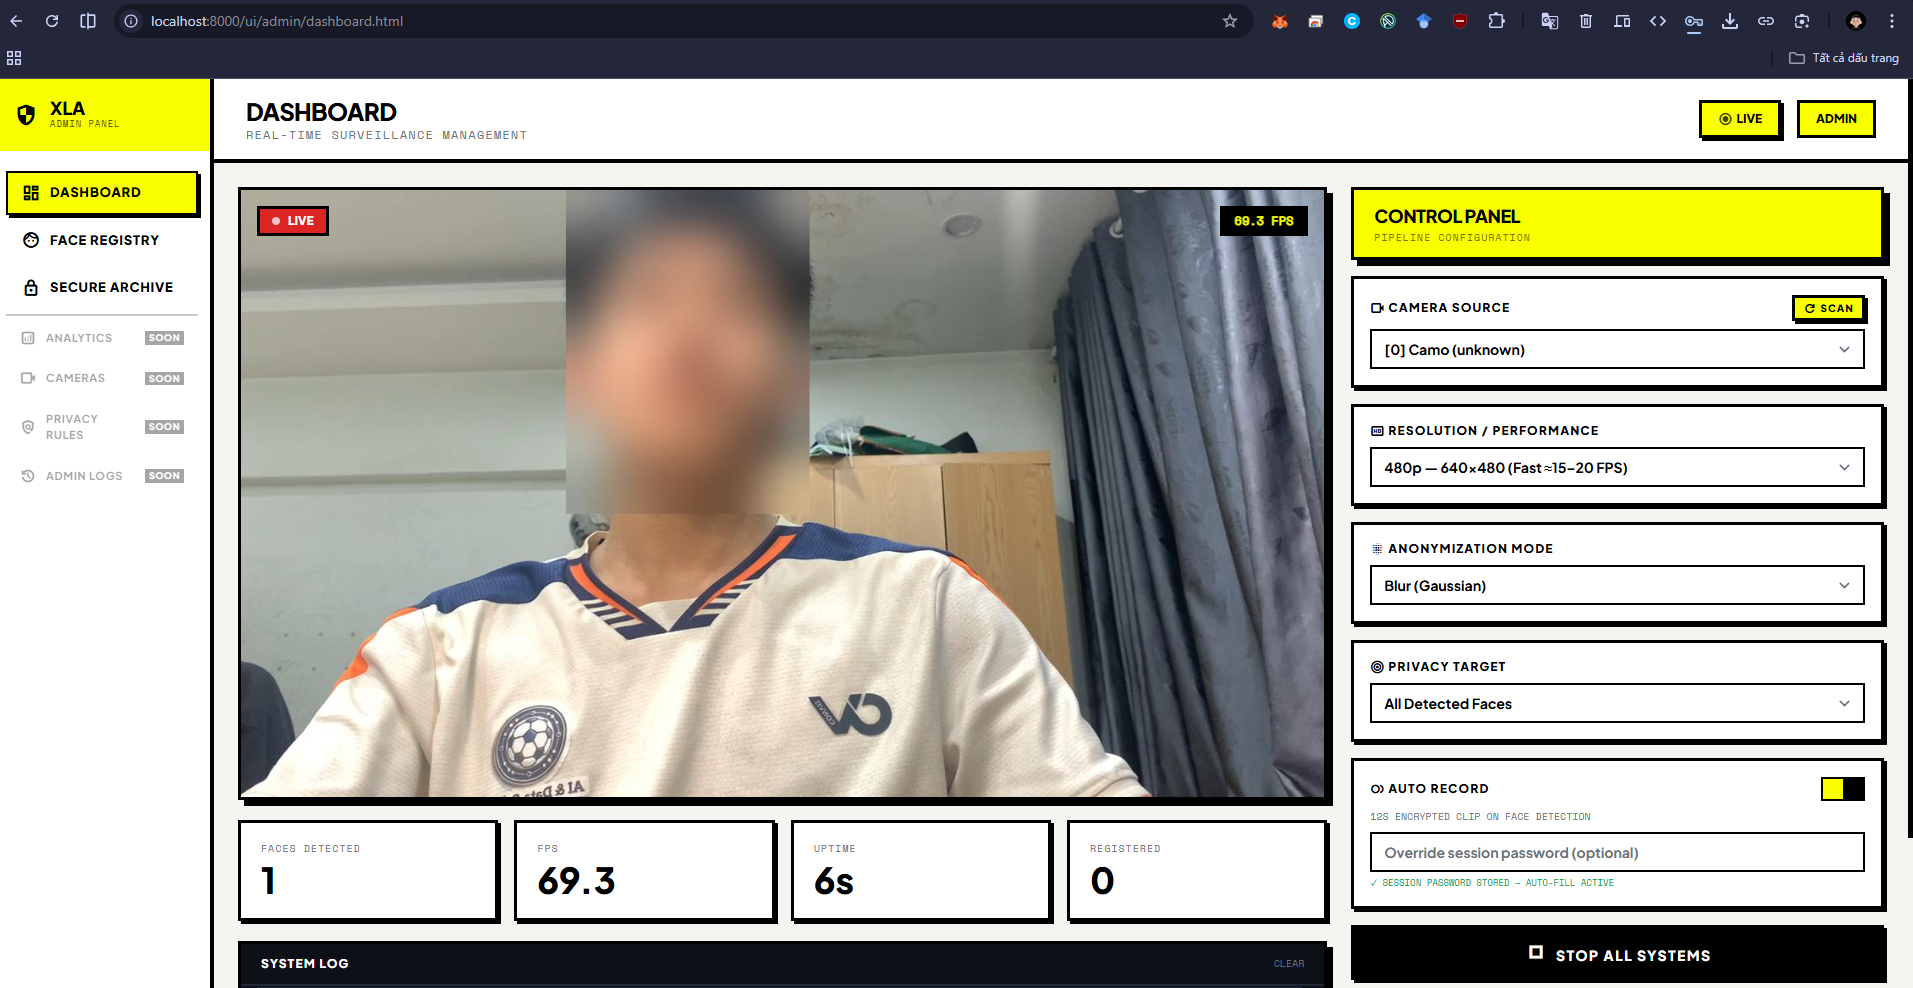
\includegraphics[width=\linewidth]{blur.png}\\[2pt]{\footnotesize\textbf{blur} --- Gaussian nhẹ}
\end{minipage}\hfill
\begin{minipage}{0.3\textwidth}\centering
  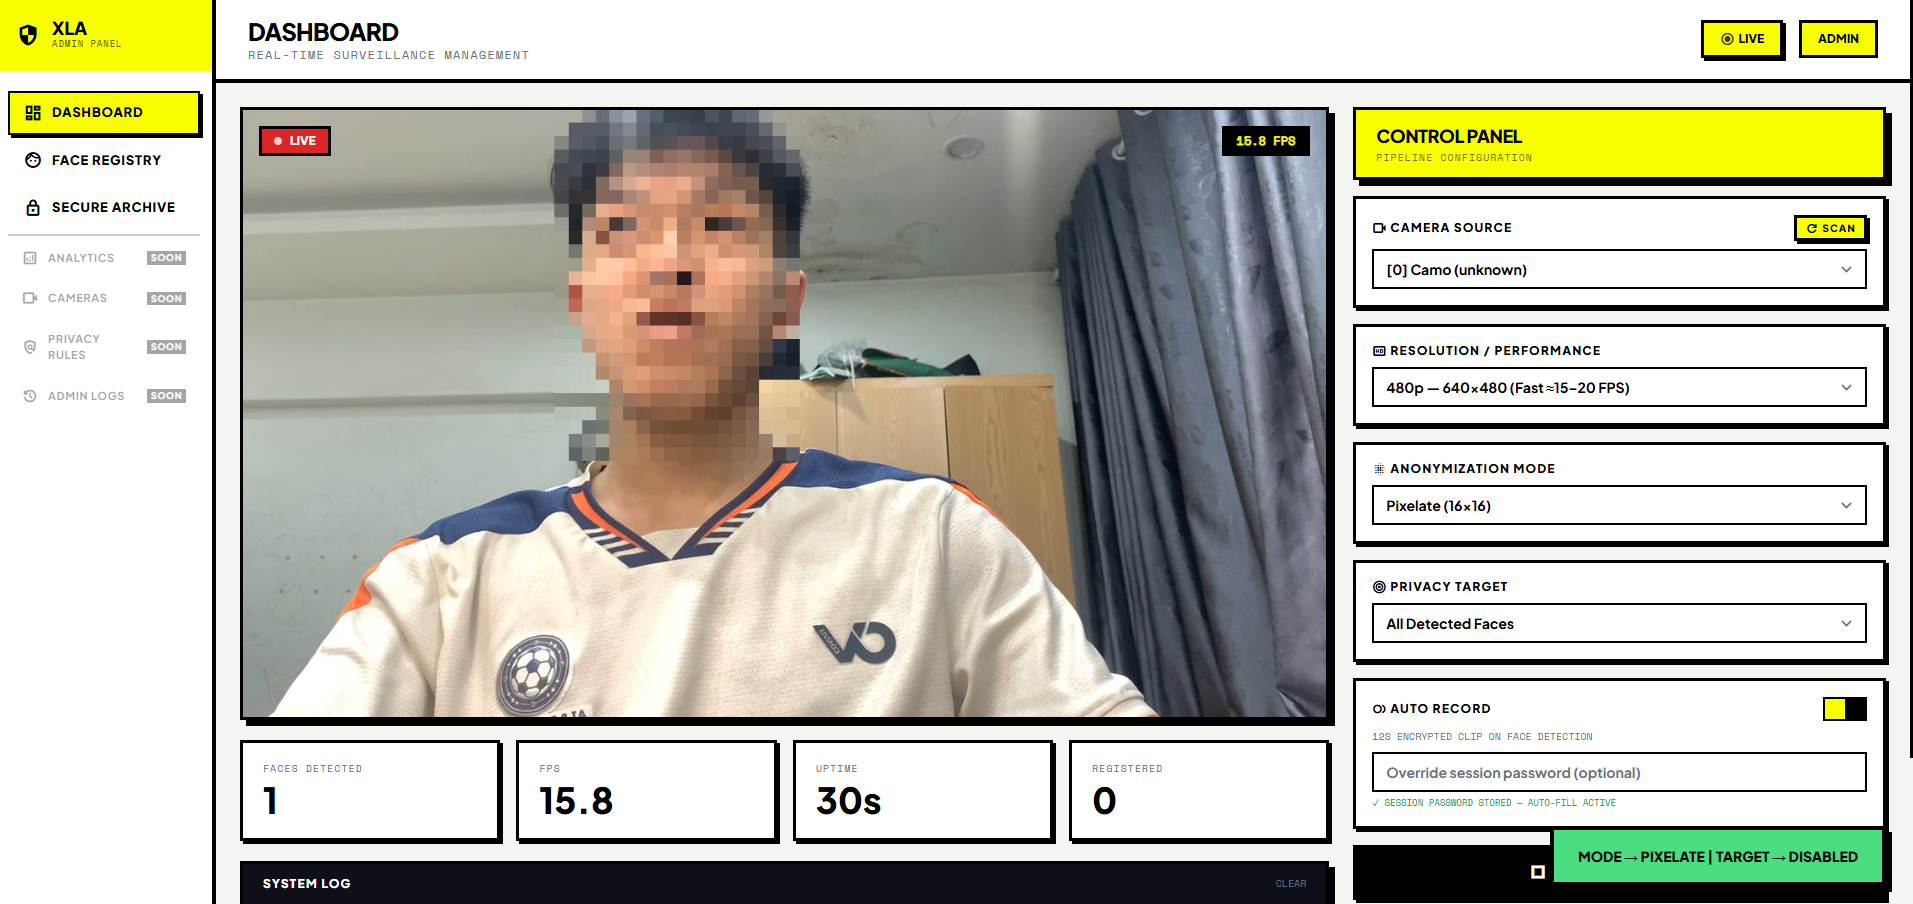
\includegraphics[width=\linewidth]{pixelate.png}\\[2pt]{\footnotesize\textbf{pixelate} --- Mosaic}
\end{minipage}\hfill
\begin{minipage}{0.3\textwidth}\centering
  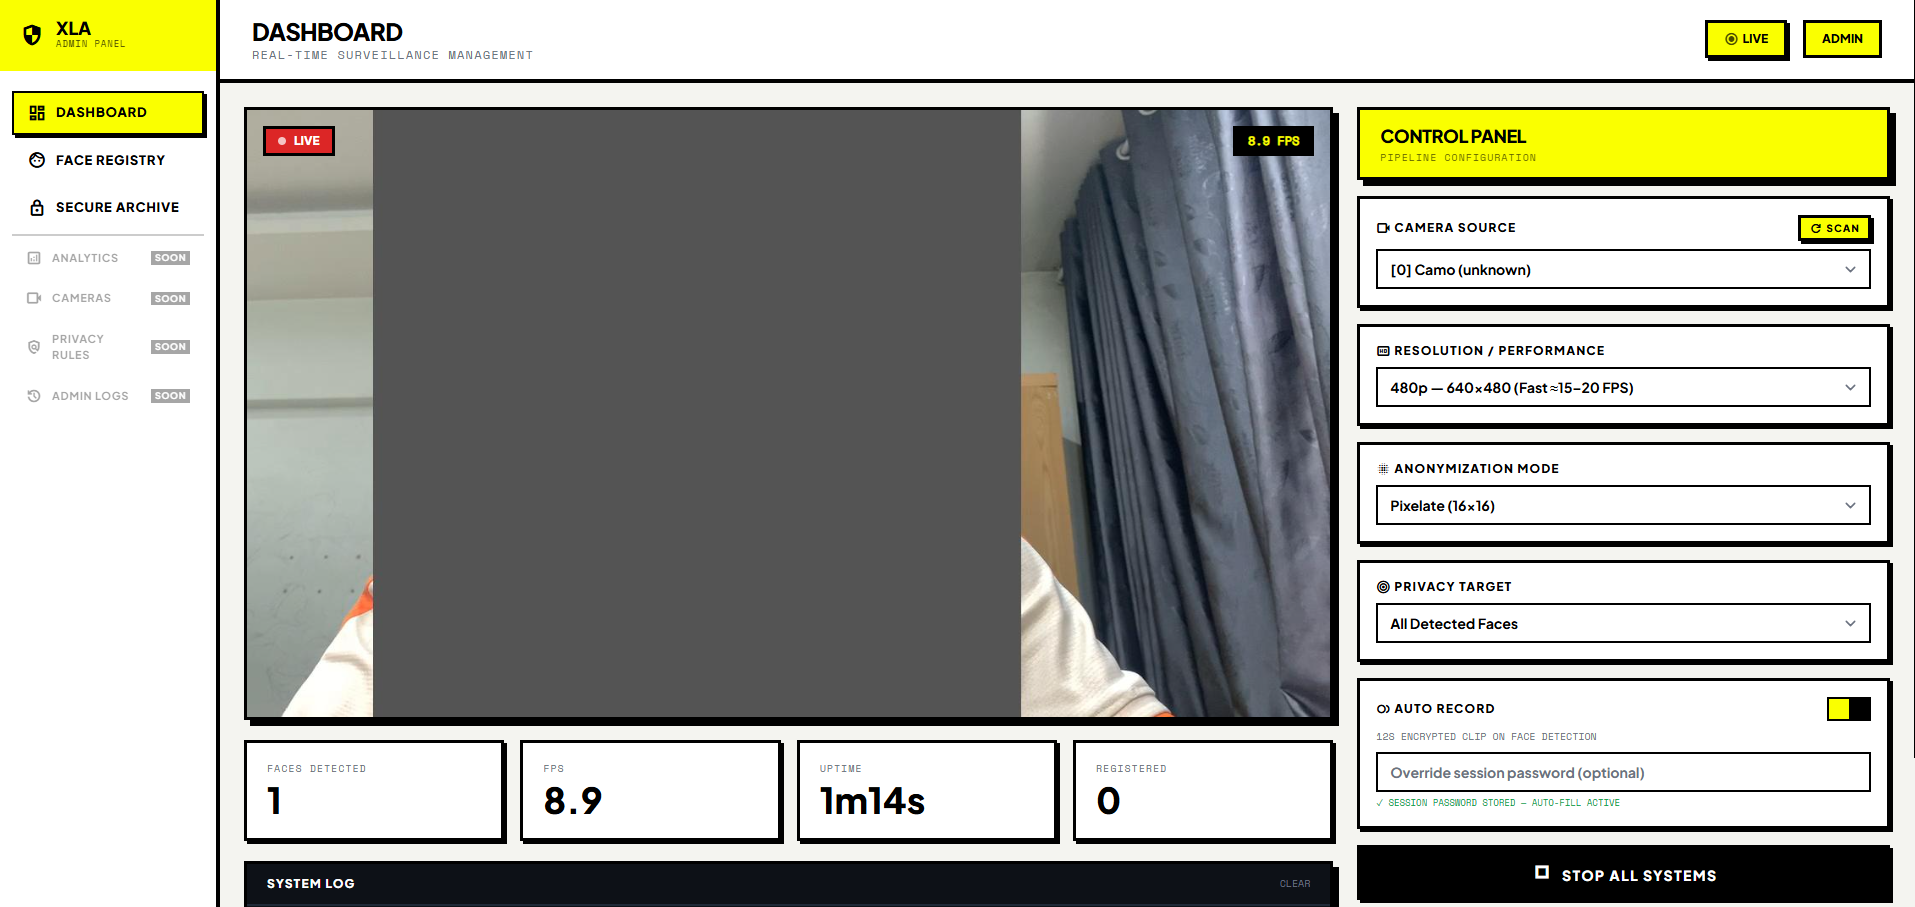
\includegraphics[width=\linewidth]{headcloak.png}\\[2pt]{\footnotesize\textbf{headcloak} --- Mix+Noise}
\end{minipage}
\\[0.3cm]
\begin{minipage}{0.3\textwidth}\centering
  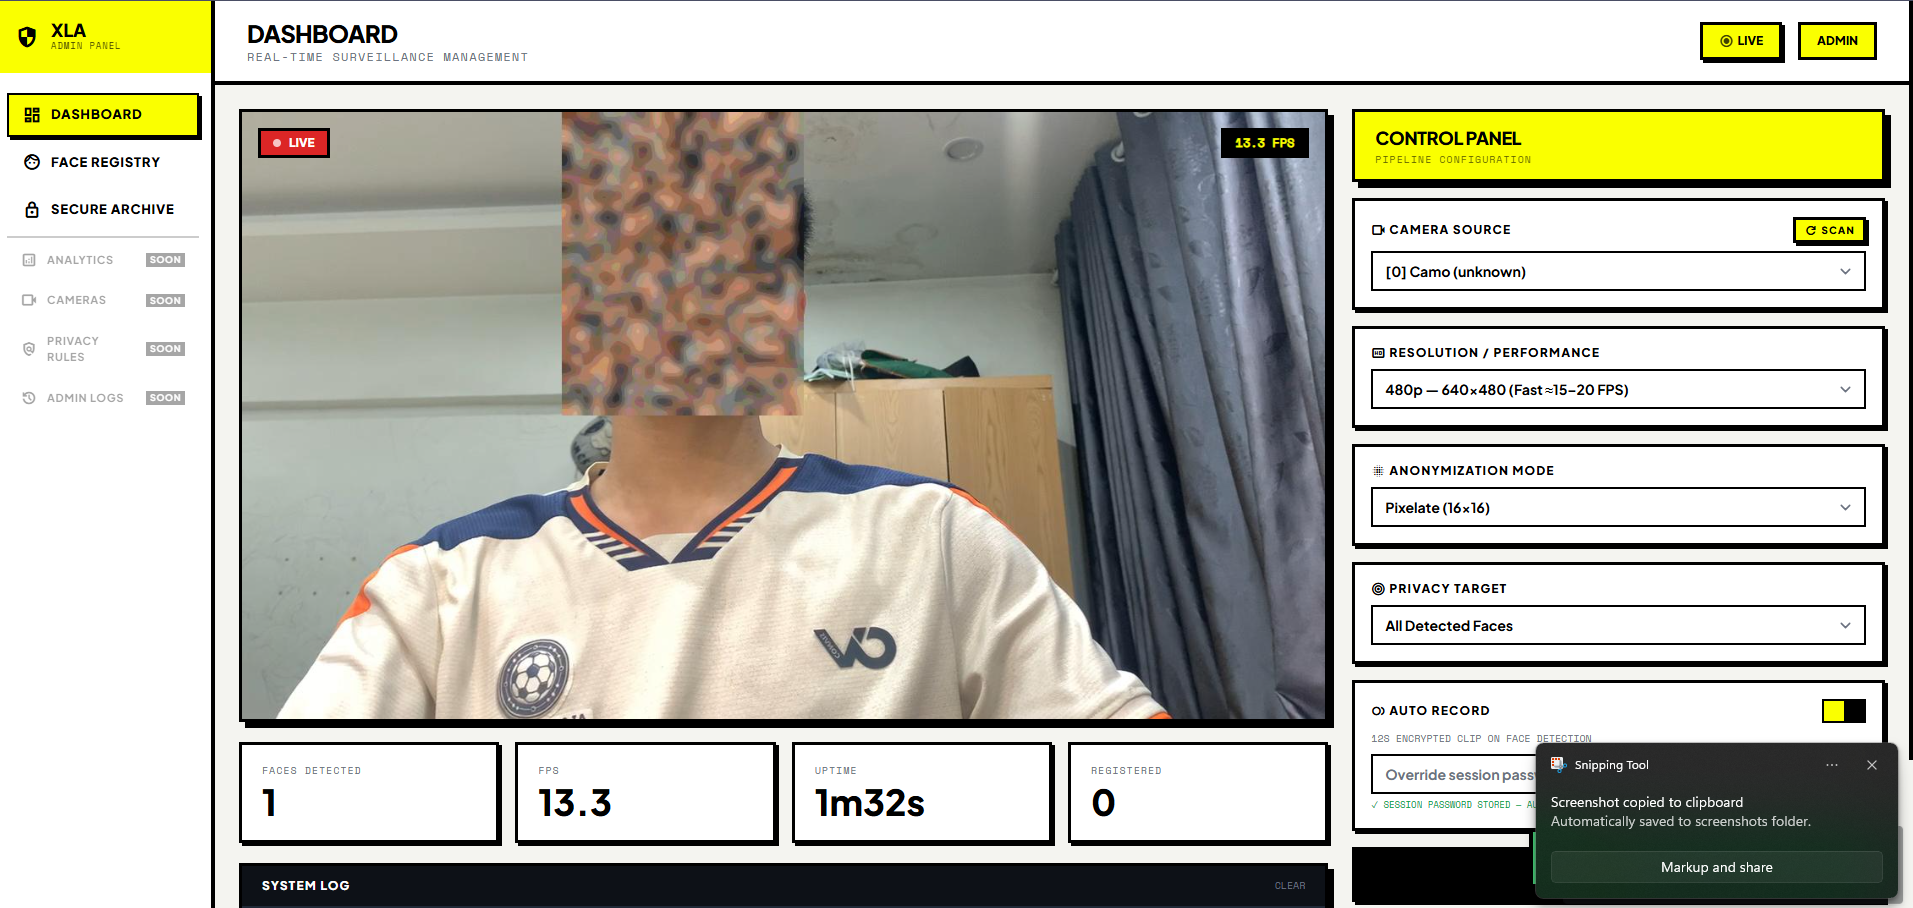
\includegraphics[width=\linewidth]{obliterate.png}\\[2pt]{\footnotesize\textbf{obliterate} --- 4-step}
\end{minipage}\hfill
\begin{minipage}{0.3\textwidth}\centering
  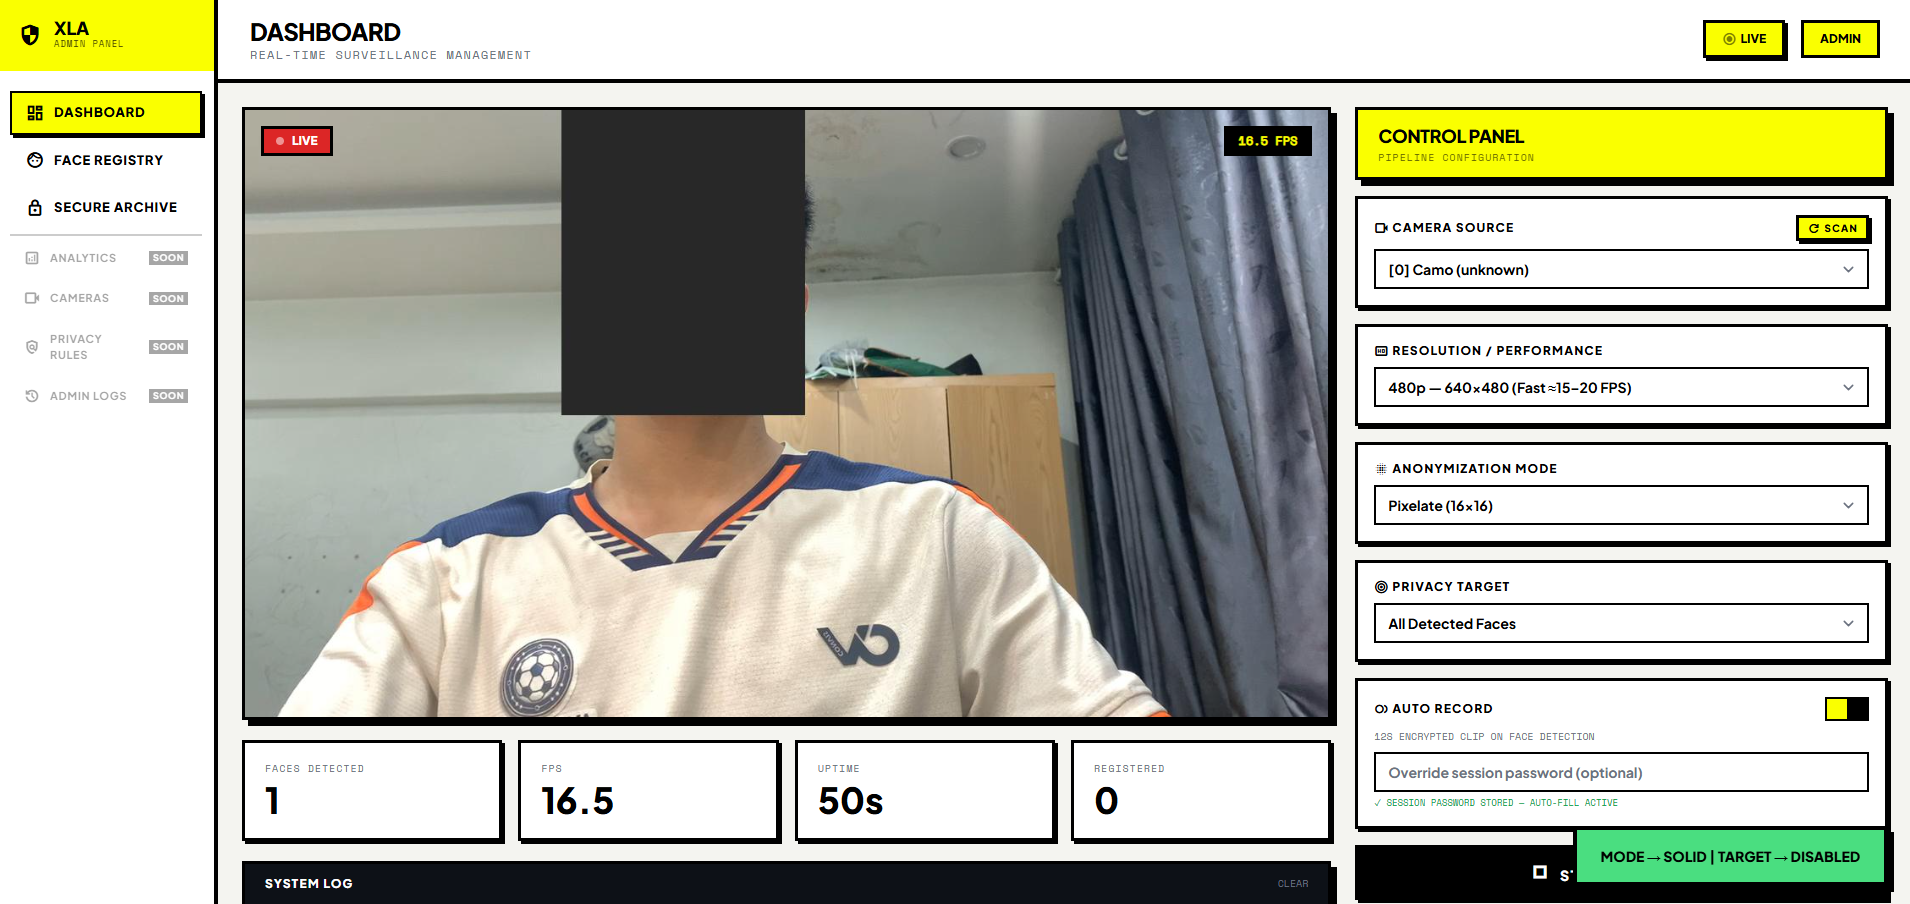
\includegraphics[width=\linewidth]{solid.png}\\[2pt]{\footnotesize\textbf{solid} --- Black box}
\end{minipage}\hfill
\begin{minipage}{0.3\textwidth}\centering
  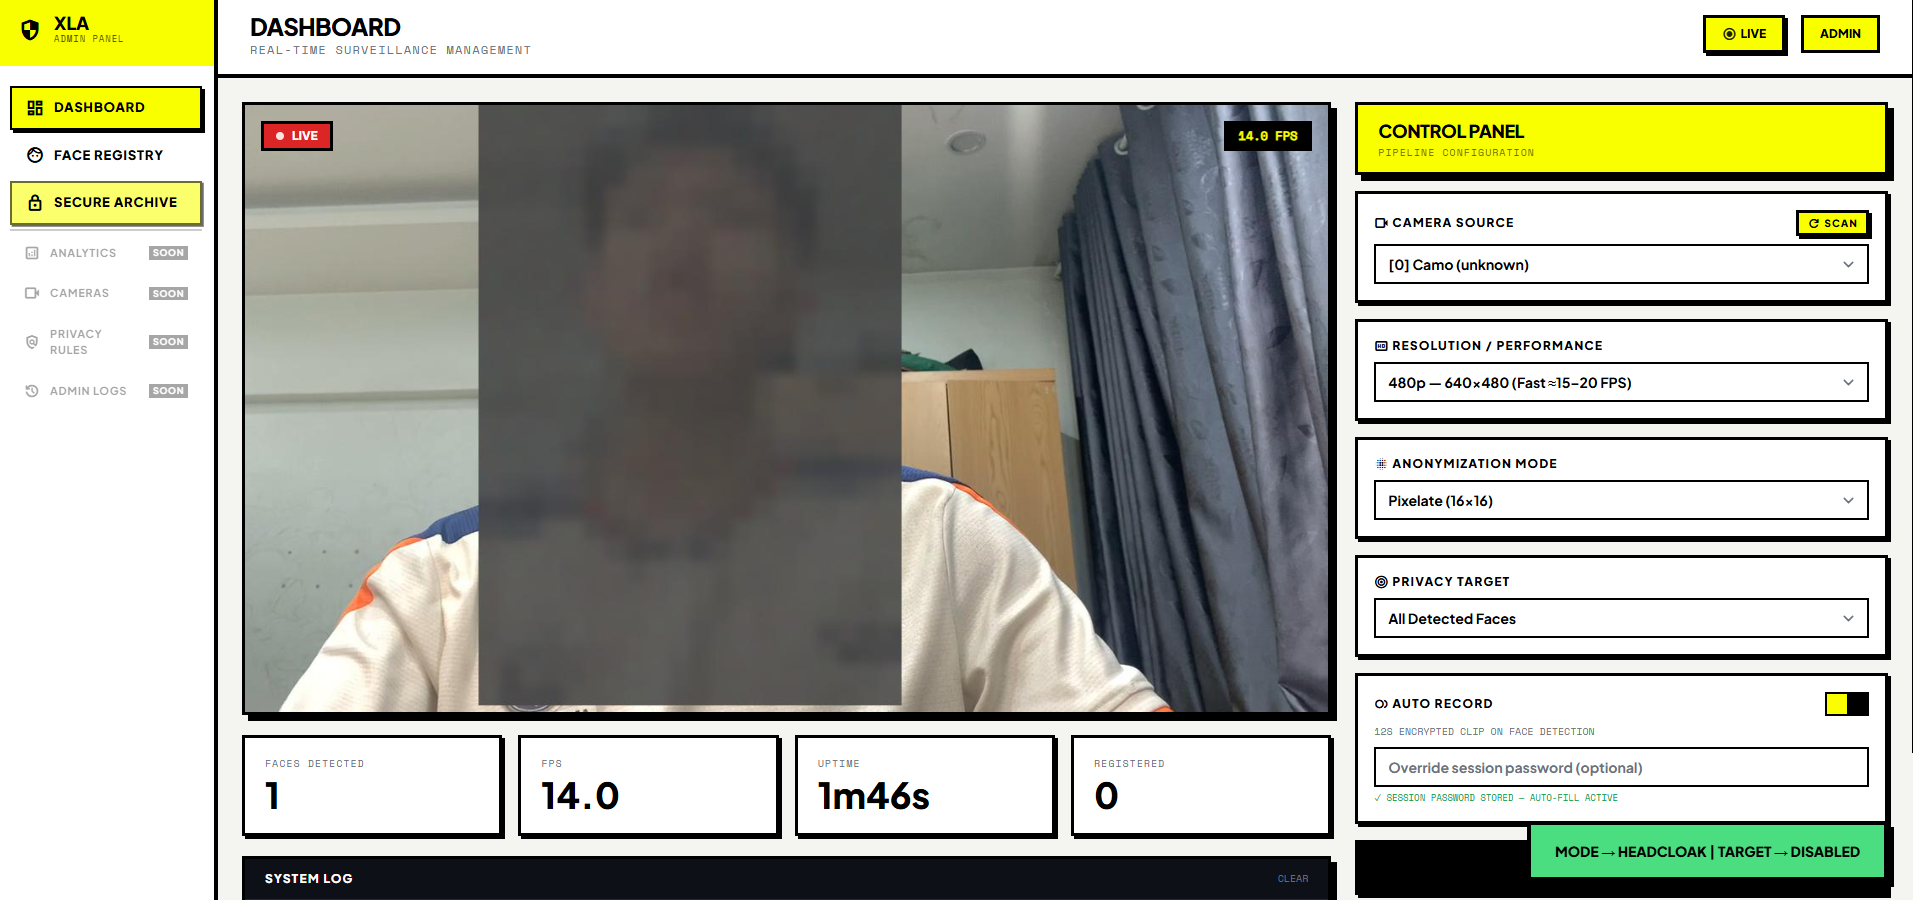
\includegraphics[width=\linewidth]{silhouette.png}\\[2pt]{\footnotesize\textbf{silhouette} --- Extreme}
\end{minipage}
\end{figure}
\end{frame}

\begin{frame}[fragile]{Chi Tiết Các Chế Độ Ẩn Danh Hoá}
\begin{columns}[T]
\column{0.52\textwidth}
\begin{tabular}{llll}
\toprule
\textbf{Mode} & \textbf{Kỹ thuật} & \textbf{CPU} & \textbf{FPS*} \\
\midrule
\texttt{blur}       & Gaussian downscale   & Thấp    & $\sim$25 \\
\texttt{pixelate}   & Bilinear + Nearest   & Rất thấp & $\sim$28 \\
\texttt{solid}      & Constant fill        & Tối thiểu & $\sim$30+ \\
\texttt{headcloak}  & Mix+Noise+GBlur      & Trung bình & $\sim$18 \\
\texttt{neckup}     & Expand+Cloak         & TB-Cao  & $\sim$15 \\
\texttt{obliterate} & 4-step pipeline      & Cao     & $\sim$12 \\
\texttt{silhouette} & Extreme cloak        & Rất cao & $\sim$8  \\
\bottomrule
\multicolumn{4}{l}{\scriptsize *CPU mid-range, proc\_width=640}
\end{tabular}

\vspace{0.5em}
\begin{block}{\faExpand\ Expand Box}
\footnotesize
\texttt{headcloak} expand trước khi blur:\\
\textbullet\ Left/Right: $\pm35\%$--$70\%$ width\\
\textbullet\ Top: $+70\%$--$120\%$ (tóc)\\
\textbullet\ Bottom: $+25\%$--$50\%$ (cằm)\\
$\Rightarrow$ không còn thấy tai, tóc, jawline
\end{block}

\column{0.44\textwidth}
\begin{lstlisting}[language=Python,
  caption={privacy.py --- obliterate}]
def _obliterate_features(roi,...):
  """4-step, IRREVERSIBLE"""
  h, w = roi.shape[:2]

  # 1. Compress to 8% - destroy detail
  small = cv2.resize(roi,
    (int(w*0.08), int(h*0.08)),
    interpolation=INTER_AREA)
  work = cv2.resize(small, (w, h),
    interpolation=INTER_NEAREST)

  # 2. Scramble 12x12 blocks
  work = _scramble_blocks(
    work, block_size=12, seed=1337)

  # 3. Heavy Gaussian blur (35)
  work = cv2.GaussianBlur(
    work, (35,35), 0)

  # 4. Quantize to 10 colors
  work = _quantize_colors(
    work, levels=10)
  return work
\end{lstlisting}
\end{columns}
\end{frame}

% ================================================================
%  SECTION 4: BACKEND & PIPELINE
% ================================================================
\section{Backend \& Live Pipeline}

\begin{frame}{FastAPI Backend --- REST + WebSocket + SSE}
\begin{columns}[T]
\column{0.48\textwidth}
\begin{block}{\faNetworkWired\ Endpoint Groups}
\footnotesize\renewcommand{\arraystretch}{1.25}
\begin{tabular}{ll}
\texttt{GET /health}           & Server status \\
\texttt{GET /presets}          & 4 config presets \\
\hline
\texttt{POST /anonymize}       & Blur ảnh upload \\
\texttt{POST /pipeline/start}  & Start live pipeline \\
\texttt{PATCH /pipeline/config} & \textbf{Hot-reload} \\
\hline
\texttt{GET /stream/mjpeg}     & MJPEG stream \\
\texttt{WS /stream/ws}         & WebSocket binary \\
\hline
\texttt{GET /members}          & List members \\
\texttt{POST /members}         & Register face \\
\hline
\texttt{GET /clips}            & List clips \\
\texttt{POST /clips/decrypt}   & Admin decrypt \\
\end{tabular}
\end{block}

\column{0.48\textwidth}
\begin{block}{\faDatabase\ 4 Preset Cấu Hình}
\footnotesize\renewcommand{\arraystretch}{1.3}
\begin{tabular}{lll}
\textbf{Preset} & \textbf{Mode} & \textbf{YOLO} \\
\hline
\texttt{fast}     & pixelate   & 416 px \\
\texttt{balanced} & headcloak  & 512 px \\
\texttt{strong}   & obliterate & 512 px \\
\texttt{strict}   & headcloak  & 416 px \\
\end{tabular}
\end{block}

\begin{block}{\faBolt\ Hot-reload Không Restart}
\footnotesize
\texttt{PATCH /pipeline/config}\\
Đổi mode / threshold / proc\_width\\
ngay trong khi đang stream.\\
$\Rightarrow$ Production-ready
\end{block}

\begin{alertblock}{\faRss\ Streaming Options}
\footnotesize
\textbullet\ \textbf{MJPEG}: \texttt{<img src="/stream/mjpeg">}\\
\textbullet\ \textbf{WebSocket}: binary frame, low-latency\\
\textbullet\ \textbf{SSE}: EventSource status updates
\end{alertblock}
\end{columns}
\end{frame}

\begin{frame}{Live Pipeline --- Luồng Xử Lý Real-time}
\begin{center}
\begin{tikzpicture}[node distance=0.5cm and 0.75cm,
    scale=0.78, every node/.style={scale=0.78}]
  \node[module, minimum width=2cm] (cam)    {\faCamera\\Camera};
  \node[module, right=of cam, minimum width=2.3cm]    (fr)     {Frame\\Reader\\Thread};
  \node[module, right=of fr, minimum width=2.3cm]     (yolo)   {YOLOv11\\detect\\\_every=2};
  \node[module, right=of yolo, minimum width=2.3cm]   (smooth) {BBox\\Smoother\\EMA $\alpha$=0.7};
  \node[module, right=of smooth, minimum width=2.3cm] (if)     {InsightFace\\buffalo\_l\\512-dim};

  \node[module, below=1.5cm of yolo, xshift=1.2cm, minimum width=2.4cm] (db)
    {FamilyDB\\match()\\cosine};
  \node[greenmod, left=0.7cm of db, minimum width=2.4cm] (anon)
    {anonymize\\\_faces()\\7 modes};
  \node[highlight, right=0.7cm of db, minimum width=2.4cm] (rec)
    {ClipRecorder\\AES-256\\GCM};

  \draw[arrow] (cam) -- (fr);
  \draw[arrow] (fr)  -- (yolo);
  \draw[arrow] (yolo) -- (smooth);
  \draw[arrow] (smooth) -- (if);
  \draw[arrow] (if) -- ++(0,-0.95) -| (db);
  \draw[arrow] (db) -- (anon);
  \draw[arrow] (db) -- (rec);
  \draw[->, dashed, gray, >=Stealth] (anon) -- ++(-2.8,0)
    node[left, font=\tiny] {MJPEG / WS};
  \draw[->, dashed, accent, >=Stealth] (rec) -- ++(2.2,0)
    node[right, font=\tiny\color{accent}] {.enc + .mp4};
\end{tikzpicture}
\end{center}

\vspace{-0.2em}
\begin{columns}[T]
\column{0.32\textwidth}
\begin{block}{\faCogs\ FrameReader Thread}
\footnotesize
\texttt{cv2.VideoCapture.read()} blocking.\\
Thread riêng → frame luôn fresh,\\
không stale khi YOLO đang chạy.
\end{block}

\column{0.32\textwidth}
\begin{block}{\faSlidersH\ BBox Smoother}
\footnotesize
EMA: $\hat{b}_t = \alpha b_t + (1-\alpha)\hat{b}_{t-1}$\\
$\alpha = 0.7$ — responsive + mượt.\\
Loại bỏ jitter frame-by-frame.
\end{block}

\column{0.32\textwidth}
\begin{block}{\faBell\ detect\_every=2}
\footnotesize
YOLO 1 lần / 2 frame.\\
Frame bỏ qua dùng lại bbox cũ.\\
$\Rightarrow$ Giảm 50\% compute cost.
\end{block}
\end{columns}
\end{frame}

% ================================================================
%  SECTION 5: SECURITY
% ================================================================
\section{Bảo Mật}

\begin{frame}{AES-256-GCM --- Mã Hoá Video Gốc}
\begin{columns}[T]
\column{0.5\textwidth}
\begin{center}
\begin{tikzpicture}[node distance=0.55cm and 0.9cm,
    scale=0.80, every node/.style={scale=0.80}]
  \node[module, minimum width=2.8cm] (frame)
    {Raw Frames\\từ camera};
  \node[module, right=0.8cm of frame, minimum width=2.8cm] (pack)
    {\_pack\_frames()\\JPEG 90 quality};
  \node[highlight, right=0.8cm of pack, minimum width=2.8cm] (aes)
    {AES-256-GCM\\encrypt()};

  \node[module, below=1.1cm of frame, minimum width=2.8cm] (salt)
    {secrets.token\_bytes(32)\\Per-clip Salt};
  \node[module, below=1.1cm of pack, minimum width=2.8cm] (pbkdf2)
    {PBKDF2-SHA256\\390\,000 rounds};
  \node[highlight, right=0.8cm of aes, minimum width=2.8cm] (enc)
    {.enc file\\{\tiny[32B salt][12B nonce]}\\{\tiny ciphertext+tag}};

  \draw[arrow] (frame) -- (pack);
  \draw[arrow] (pack)  -- (aes);
  \draw[arrow] (salt)  -- (pbkdf2);
  \draw[arrow] (pbkdf2) -- (aes) node[midway, right, font=\tiny] {32B key};
  \draw[arrow] (aes) -- (enc);
  \node[font=\tiny, below=0.05cm of salt] {password admin};
\end{tikzpicture}
\end{center}

\column{0.46\textwidth}
\begin{block}{\faKey\ Per-clip Salt (32 bytes)}
\footnotesize
Mỗi clip = 1 salt 32B ngẫu nhiên.\\
Cùng password → \textbf{khác key}.\\
Lộ 1 clip ≠ lộ tất cả clip.
\end{block}

\begin{block}{\faLock\ AES-256-GCM}
\footnotesize
\textbf{Authenticated Encryption}.\\
Auth Tag 128-bit tích hợp.\\
Sửa 1 bit ciphertext → decrypt fail.\\
$\not\Rightarrow$ dữ liệu sai mà không hay.
\end{block}

\begin{block}{\faClock\ PBKDF2-SHA256}
\footnotesize
390\,000 rounds (OWASP 2023 min).\\
Brute-force password 8 ký tự:\\
$\approx$ \textbf{hàng trăm nghìn năm} với GPU.
\end{block}
\end{columns}
\end{frame}

\begin{frame}[fragile]{Admin Authentication --- PBKDF2 + Timing-safe}
\begin{columns}[T]
\column{0.52\textwidth}
\begin{lstlisting}[language=Python,
  caption={admin\_auth.py}]
_ITERATIONS = 390_000  # OWASP 2023

def _pbkdf2(password, salt,
            iters=_ITERATIONS):
    kdf = PBKDF2HMAC(
        algorithm=hashes.SHA256(),
        length=32,   # 256-bit key
        salt=salt,
        iterations=iters,
    )
    return kdf.derive(
        password.encode("utf-8"))

def _ct_equal(a: bytes, b: bytes):
    """Prevent Timing Attack."""
    # Python '==' stops at 1st diff ->
    # attacker measures response time
    # -> guesses chars byte-by-byte
    # hmac.compare_digest: CONSTANT TIME
    return hmac.compare_digest(a, b)
\end{lstlisting}

\column{0.44\textwidth}
\begin{block}{\faDatabase\ Credentials File}
\footnotesize
\begin{lstlisting}[numbers=none]
{
  "salt": "aGVsbG8h...",
  "hash": "c2VjcmV0...",
  "iterations": 390000
}
\end{lstlisting}
\textbf{Không có plaintext password.}\\
Ngay cả developer cũng không biết.
\end{block}

\begin{alertblock}{\faExclamationTriangle\ Timing Attack}
\footnotesize
\texttt{a == b}: dừng ở byte sai đầu tiên\\
→ thời gian response leak thông tin\\
\smallskip
\texttt{hmac.compare\_digest}: luôn compare hết\\
→ constant-time, không leak
\end{alertblock}

\begin{block}{\faLock\ OWASP Compliance}
\footnotesize
\textbullet\ Broken Access Control: role check\\
\textbullet\ Crypto Failure: AES-256-GCM\\
\textbullet\ Injection: FastAPI type validation\\
\textbullet\ Auth Failure: PBKDF2 + timing-safe
\end{block}
\end{columns}
\end{frame}

% ================================================================
%  SECTION 6: DEMO & KẾT QUẢ
% ================================================================
\section{Demo \& Kết Quả}

\begin{frame}{Giao Diện Admin Dashboard}
\begin{columns}[T]
\column{0.62\textwidth}
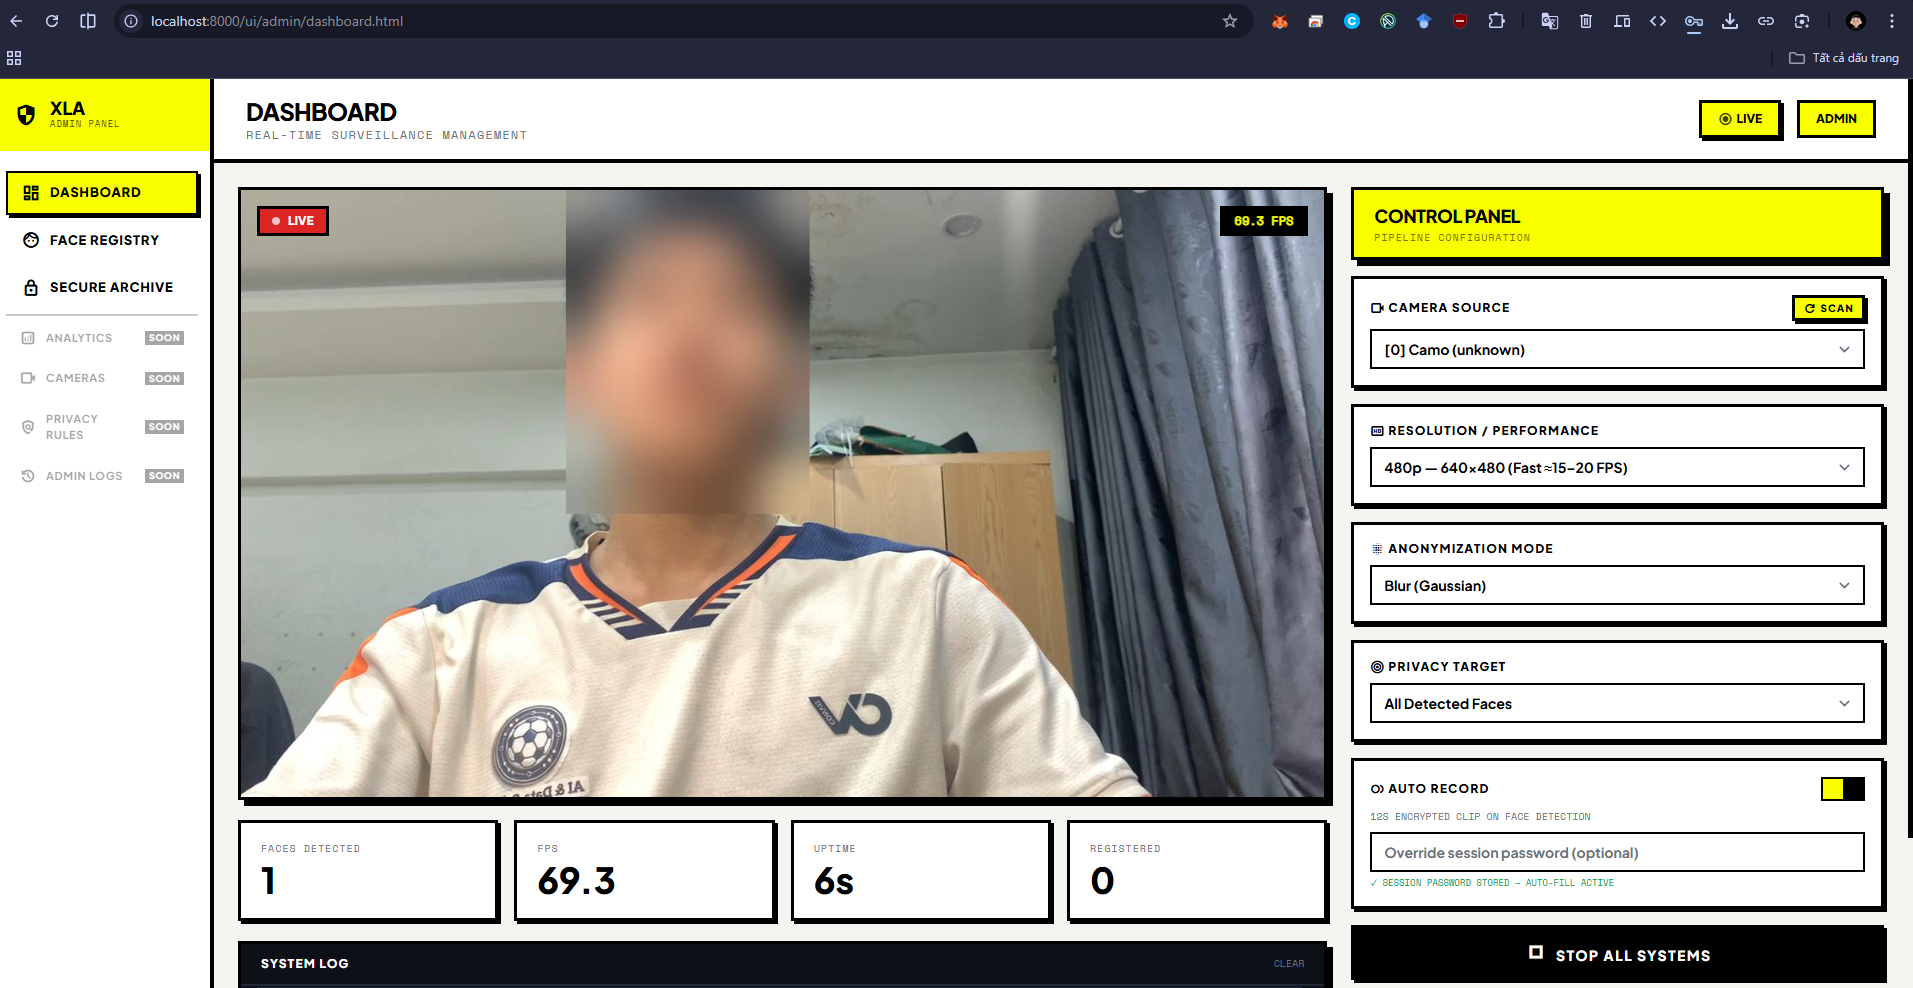
\includegraphics[width=\linewidth]{admin_dashboard.png}

\column{0.34\textwidth}
\begin{block}{\faDesktop\ Admin Dashboard}
\footnotesize
\textbf{URL:} \texttt{/admin/dashboard.html}
\begin{itemize}
  \item Xem live stream video đã blur
  \item Điều khiển pipeline (Start / Stop)
  \item Đổi chế độ ẩn danh on-the-fly
  \item Xem FPS, latency realtime
  \item Quản lý thành viên gia đình
\end{itemize}
\end{block}

\begin{alertblock}{\faLock\ Yêu cầu đăng nhập}
\footnotesize
Chỉ Admin mới truy cập được.\\
Guest → redirect đăng nhập.
\end{alertblock}
\end{columns}
\end{frame}

\begin{frame}{Giao Diện User Portal}
\begin{columns}[T]
\column{0.62\textwidth}
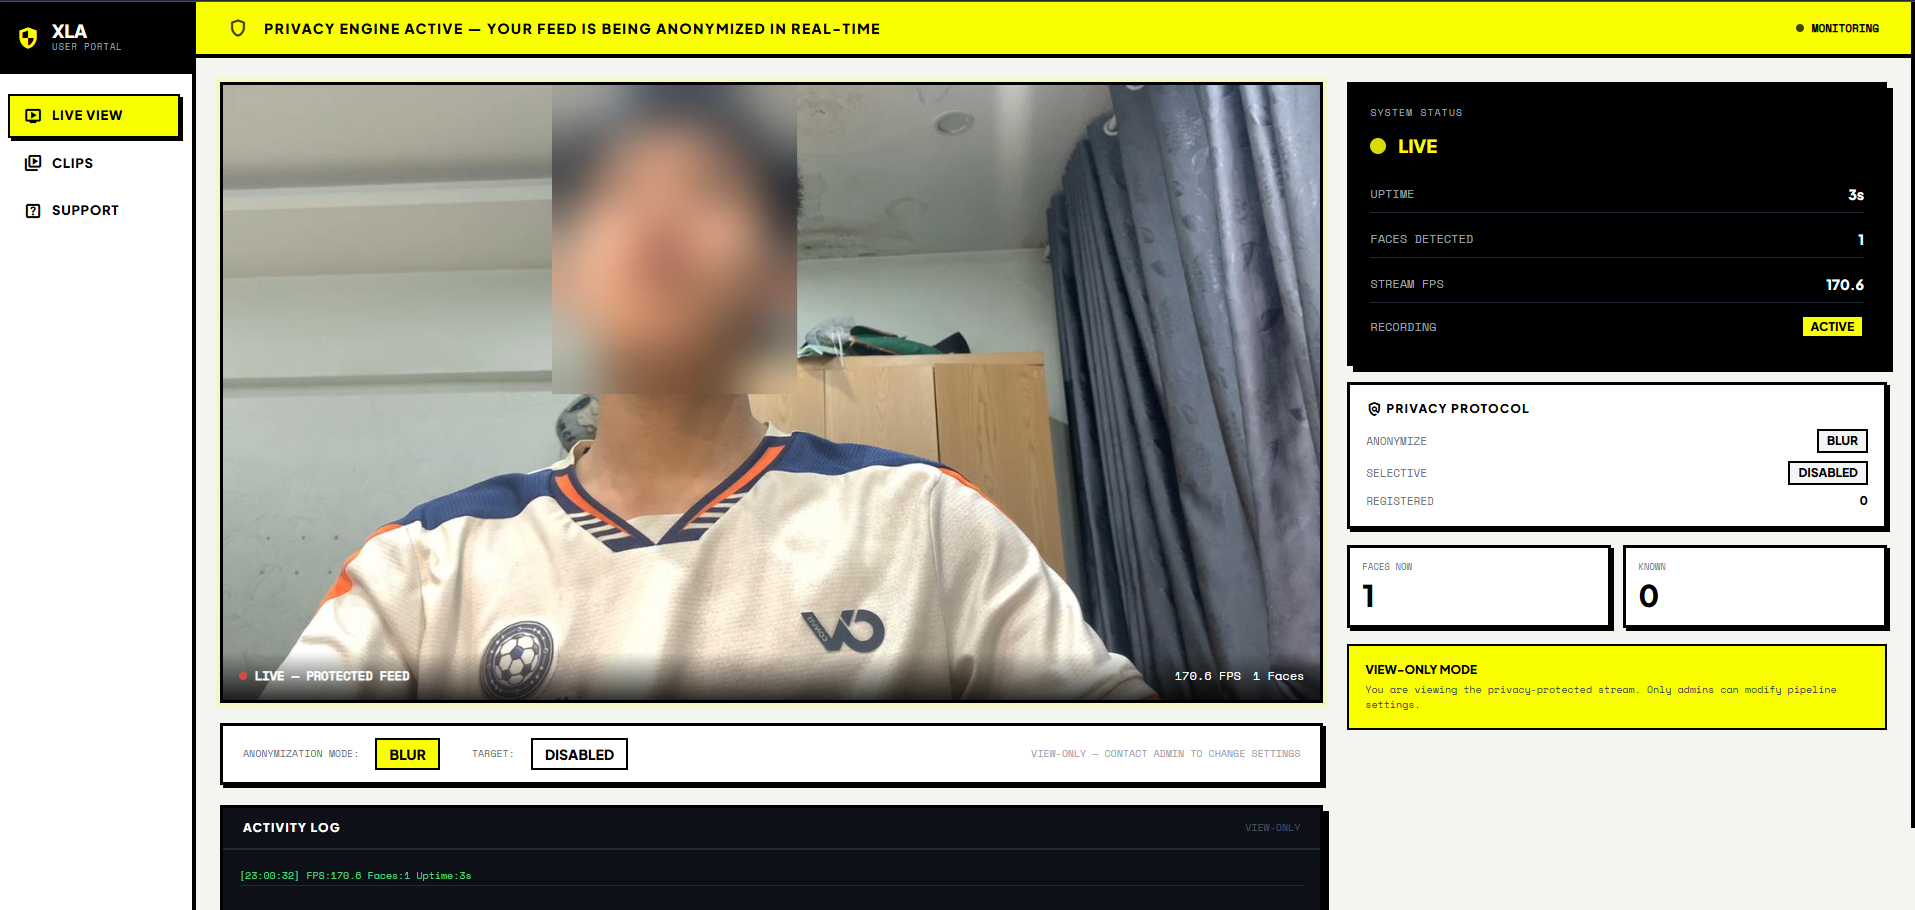
\includegraphics[width=\linewidth]{user_portal.png}

\column{0.34\textwidth}
\begin{block}{\faEye\ User Portal}
\footnotesize
\textbf{URL:} \texttt{/user/live-portal.html}
\begin{itemize}
  \item Xem stream video \textbf{đã ẩn danh}
  \item \textbf{Không cần đăng nhập}
  \item Khuôn mặt người lạ đã bị che
  \item Thành viên gia đình: hiển thị tên
  \item Không thể xem video gốc
\end{itemize}
\end{block}

\begin{block}{\faUsers\ Phân quyền}
\footnotesize
\begin{tabular}{ll}
\textbf{Role} & \textbf{Quyền} \\
\hline
Admin & Full control \\
User  & View only \\
Guest & Public stream \\
\end{tabular}
\end{block}
\end{columns}
\end{frame}

\begin{frame}{Kết Quả Benchmark}
\begin{columns}[T]
\column{0.5\textwidth}
\begin{block}{\faChartBar\ FPS Theo Chế Độ (CPU mid-range)}
\begin{center}
\begin{tikzpicture}[scale=0.75]
\begin{scope}[xscale=0.095, yscale=0.065]
  \draw[->] (0,0) -- (75,0) node[right]{\tiny FPS};
  \draw[->] (0,0) -- (0,58);

  \foreach \name/\y/\fps/\col in {
    {silhouette}/5/8.9/purple!60,
    {solid}/13/16.5/gray!70,
    {obliterate}/21/13.3/red!60,
    {headcloak}/29/14.0/orange!70,
    {pixelate}/37/15.8/teal!60,
    {blur}/45/69.3/blue!60
  }{
    \fill[\col] (0,\y) rectangle (\fps,{\y+6});
    \node[left, font=\tiny] at (-1,{\y+3}) {\name};
    \node[right, font=\tiny\bfseries] at (\fps,{\y+3}) {\fps};
  }
\end{scope}
\end{tikzpicture}
\end{center}
\end{block}

\column{0.46\textwidth}
\begin{block}{\cmark\ Nhận xét}
\footnotesize
\begin{itemize}
  \item \texttt{blur}: $\sim$\textbf{69 FPS} --- cực kỳ nhẹ
  \item \texttt{pixelate}: $\sim$\textbf{16 FPS} --- khá nhanh
  \item \texttt{headcloak}: $\sim$\textbf{14 FPS} --- mặc định
  \item \texttt{obliterate}: $\sim$\textbf{13 FPS} --- rất mạnh
  \item \texttt{silhouette}: $\sim$\textbf{9 FPS} --- cực mạnh
  \item Chạy \textbf{CPU} (không cần GPU)
\end{itemize}
\end{block}

\begin{block}{\cmark\ Nhận diện}
\footnotesize
\begin{itemize}
  \item 2 thành viên đăng ký: \textbf{nhận đúng}
  \item Cosine threshold 0.35 hiệu quả
  \item Không false positive trong test
  \item 100 mẫu/người: embedding ổn định
\end{itemize}
\end{block}
\end{columns}
\end{frame}

% ================================================================
%  SECTION 7: KẾT LUẬN
% ================================================================
\section{Kết Luận}

\begin{frame}{Kết Quả Đạt Được}
\begin{columns}[T]
\column{0.48\textwidth}
\begin{block}{\cmark\ Privacy (Đạt)}
\begin{itemize}\footnotesize
  \item 7 chế độ ẩn danh từ nhẹ đến cực mạnh
  \item Khuôn mặt người lạ: ẩn danh hoàn toàn
  \item Thành viên đã đăng ký: không bị che
  \item Hot-reload mode không cần restart
  \item Hỗ trợ ``expand box'' che cả tóc/tai
\end{itemize}
\end{block}

\begin{block}{\cmark\ Security (Đạt)}
\begin{itemize}\footnotesize
  \item AES-256-GCM: mã hoá + authenticated
  \item PBKDF2-SHA256 390\,000 iter (OWASP)
  \item Per-clip salt: không reuse key bao giờ
  \item Constant-time compare: no timing leak
  \item Zero knowledge of plaintext password
\end{itemize}
\end{block}

\column{0.48\textwidth}
\begin{block}{\cmark\ Detection \& Recognition (Khoa)}
\begin{itemize}\footnotesize
  \item YOLOv11n-face: nhẹ, nhanh, chính xác
  \item InsightFace buffalo\_l: 512-dim embedding
  \item Vectorized batch matching O(n)
  \item BBox EMA smoother: loại bỏ jitter
  \item 2 thành viên, 100 mẫu/người
\end{itemize}
\end{block}

\begin{block}{\cmark\ Backend \& UI (Khánh)}
\begin{itemize}\footnotesize
  \item FastAPI REST + WebSocket + SSE
  \item MJPEG + WebSocket dual streaming
  \item 4 preset cấu hình sẵn sàng dùng
  \item 6 trang HTML, responsive
  \item Phân quyền Admin / User / Guest
\end{itemize}
\end{block}
\end{columns}
\end{frame}

\begin{frame}{Hạn Chế \& Hướng Phát Triển}
\begin{columns}[T]
\column{0.48\textwidth}
\begin{alertblock}{\faTimes\ Hạn chế hiện tại}
\begin{itemize}\footnotesize
  \item Chưa có GPU acceleration\\
        (CPU-only, FPS bị giới hạn)
  \item Chỉ 2 thành viên được đăng ký
  \item Không có audit log
  \item Chưa data retention policy
  \item Khánh chưa được đăng ký vào DB\\
        (minh chứng cho demo)
\end{itemize}
\end{alertblock}

\column{0.48\textwidth}
\begin{block}{\faArrowRight\ Hướng mở rộng}
\begin{itemize}\footnotesize
  \item GPU inference (CUDA / TensorRT)
  \item Tích hợp nhiều camera đồng thời
  \item Key Escrow / Shamir Secret Sharing
  \item Audit log + compliance dashboard
  \item Cloud deployment + mobile app
  \item Threshold calibration tự động
  \item Consent management (GDPR Art.7)
\end{itemize}
\end{block}
\end{columns}

\vspace{0.4em}
\begin{block}{\faQuestionCircle\ Câu hỏi thường gặp}
\footnotesize
\begin{tabular}{ll}
\textbf{Q: Quên password?} & Không recover được --- by design. Production: Key Escrow. \\
\textbf{Q: AES-GCM vs CBC?} & GCM = Authenticated Encryption. CBC không verify integrity. \\
\textbf{Q: GDPR compliance?} & Privacy by Design Art.25. Cần thêm: audit log, consent, retention.\\
\end{tabular}
\end{block}
\end{frame}

% ================================================================
%  FINAL SLIDE
% ================================================================
\begin{frame}[plain]
\begin{tikzpicture}[remember picture, overlay]
  \fill[primary] (current page.north west)
    rectangle ([yshift=-0.5\paperheight] current page.north east);

  \node[text=white, font=\LARGE\bfseries, anchor=center]
    at ([yshift=-1.8cm] current page.north)
    {Cảm ơn Thầy/Cô đã lắng nghe!};

  \node[text=white!85, font=\large, anchor=center]
    at ([yshift=-2.9cm] current page.north)
    {XLA Face Privacy System};

  \node[text=white!65, font=\normalsize, anchor=center]
    at ([yshift=-3.7cm] current page.north)
    {Privacy by Default · Evidence on Demand · AES-256-GCM};
\end{tikzpicture}

\vspace{4.8cm}
\begin{columns}[c]
\column{0.55\textwidth}
\begin{block}{\faUsers\ Nhóm thực hiện}
\footnotesize\renewcommand{\arraystretch}{1.5}
\begin{tabular}{lll}
\textcolor{accent}{\textbf{Đạt}} & Leader & AES-256-GCM · PBKDF2 · Blur Engine \\
\textbf{Khánh} & Backend & FastAPI · Pipeline · Streaming \\
\textbf{Khoa} & Detection & YOLOv11 · InsightFace · DB \\
\end{tabular}
\end{block}

\column{0.38\textwidth}
\begin{block}{\faCode\ Repository}
\footnotesize
\faGithub\ \texttt{Poicitaco/XLA\_T3}\\
Branch: \texttt{feature/cipher}\\
\faServer\ \texttt{uvicorn} --- Port \texttt{8000}\\
\faPython\ Python 3.13
\end{block}
\end{columns}

\vspace{0.5em}
\begin{center}
\large\textbf{\textcolor{primary}{\faHandPointRight\ Sẵn sàng trả lời câu hỏi!}}
\end{center}
\end{frame}

\end{document}
